% =============================================================================
% CAPÍTULO IV - RESULTADOS
% =============================================================================

\cleardoublepage
\thispagestyle{empty}
\vspace*{\fill}
\begin{center}
{\Large\bfseries CAPÍTULO IV}\\[2.5cm]
{\Large\bfseries RESULTADOS}
\end{center}
\vspace*{\fill}
\clearpage

\chapter*{}
\addcontentsline{toc}{chapter}{CAPÍTULO IV -- RESULTADOS}
\setcounter{chapter}{4}
\setcounter{section}{0}
\renewcommand{\thesection}{4.\arabic{section}}
\renewcommand{\thesubsection}{4.\arabic{section}.\arabic{subsection}}

\vspace{-3cm}

\section{Producto tecnológico desarrollado}

En esta sección se presentan los resultados obtenidos a lo largo del desarrollo del proyecto tecnológico Kiddy Quiz, habiendo alcanzado los objetivos planteados mediante la aplicación de la metodología ágil de Programación Extrema (XP). A través de iteraciones cortas, retroalimentación constante por parte de los docentes especialistas y la refactorización continua del código, se garantizó la entrega de un software alineado con las necesidades educativas. La presente sección detalla lo obtenido en cada etapa, comenzando por la obtención y análisis de los requisitos, continuando con el diseño y desarrollo del sistema, y finalizando con la fase de pruebas y validación, asegurando un producto de calidad, inclusivo y funcional para entornos reales. Adicionalmente, se presenta de manera detallada la comprobación de los indicadores de evaluación definidos en la sección 3.5. El manual de funcionamiento del sistema, dada su extensión y nivel de detalle visual, ha sido incluido en el Anexo~E.

De manera general, se obtuvo una aplicación web adaptativa totalmente funcional, estructurada en dos perfiles principales: estudiante y docente. El perfil del estudiante brinda un entorno accesible donde, al iniciar sesión, el usuario visualiza sus clases y puede unirse a nuevas mediante un código de acceso. Dentro de cada clase, el estudiante puede acceder a las evaluaciones asignadas, visualizar los detalles y resultados de sus pruebas, y consultar su progreso general. Una característica destacada es la integración de inteligencia artificial generativa (Gemini), la cual interviene brindando retroalimentación motivacional al finalizar cada prueba y generando contenido de refuerzo académico para fortalecer las competencias evaluadas. Por otro lado, el perfil del docente centraliza la gestión académica, mediante un módulo robusto que permite al profesor crear clases, gestionar estudiantes y administrar listas de evaluaciones, además de proveer analíticas y reportes detallados por estudiante.

\subsection{Obtención de requisitos}

Tras realizar las entrevistas y el trabajo de validación continua con los docentes especialistas, y una vez analizada toda la información recopilada (disponible en el Anexo~A), se definió el alcance del sistema. Esta información fue complementada con los lineamientos pedagógicos extraídos de la revisión bibliográfica para asegurar un enfoque adecuado hacia los estudiantes de educación básica.

Dado que el desarrollo se rigió bajo la metodología ágil de Programación Extrema (XP), la lista de requerimientos del sistema no se estructuró de forma tradicional, sino que se documentó directamente a través de veintinueve historias de usuario. En la Tabla~\ref{tab:hu} se muestra el listado consolidado de las historias de usuario que conforman el núcleo funcional de la aplicación.

\begin{table}[H]
\centering
\caption{Historias de usuario de la aplicación web Kiddy Quiz.}
\label{tab:hu}
\begin{footnotesize}
\begin{tabularx}{\textwidth}{|L{1.7cm}|L{3.5cm}|L{1.5cm}|X|X|}
\hline
\rowcolor{tabhead}
\tabhead{ID} & \tabhead{Título} & \tabhead{Como} & \tabhead{Quiero (acción)} & \tabhead{Para (beneficio)}\\
\hline
HU-001.1-F & Inicio de sesión y redirección & Usuario & Iniciar sesión con correo y contraseña & Acceder al panel correspondiente según perfil\\
\hline
HU-001.2-F & Cierre de sesión seguro & Usuario & Cerrar sesión activa mediante un botón & Proteger la información personal\\
\hline
HU-002.1-F & Registro unificado & Docente & Crear una cuenta eligiendo rol & Acceder sin necesidad de validación adicional\\
\hline
HU-002.2-F & Creación manual de alumnos & Docente & Crear cuentas directamente para mis alumnos & Facilitar el acceso y vinculación automática\\
\hline
HU-003.1-F & Panel de tarjetas (estudiante) & Estudiante & Ver evaluaciones asignadas en tarjetas visuales & Identificar rápidamente tema y dificultad\\
\hline
HU-004.1-F & Ejecución de evaluación & Estudiante & Responder preguntas de forma secuencial & Completar la prueba en un entorno amigable\\
\hline
HU-004.2-F & Soporte de control por voz & Estudiante & Activar funciones de voz en la evaluación & Interactuar de forma sencilla y autónoma\\
\hline
HU-005.1-F & \textit{Feedback} motivacional & Estudiante & Ver puntaje, tiempo y mensaje de ánimo & Sentirse motivado a mejorar\\
\hline
HU-006.1-F & Panel de gestión (docente) & Docente & Ver mis evaluaciones creadas en tarjetas & Gestionar contenido y visibilidad\\
\hline
HU-006.2-F & Habilitación rápida & Docente & Activar o desactivar pruebas con un interruptor & Controlar el acceso al examen\\
\hline
HU-006.3-F & Estructura base de evaluación & Docente & Definir tema, descripción, dificultad y duración & Establecer la configuración\\
\hline
HU-006.4-F & Modo lúdico & Estudiante & Realizar evaluaciones en formato de juego & Aprender divirtiéndose\\
\hline
HU-006.5-F & Programación temporal & Docente & Definir fechas de inicio y fin & Planificar el calendario académico\\
\hline
HU-006.6-F & Control de versiones & Docente & Mantener historial de modificaciones & Restaurar versiones en caso de errores\\
\hline
HU-006.7-F & Evaluaciones diagnósticas & Docente & Marcar pruebas como diagnósticas iniciales & Conocer el nivel previo del estudiante\\
\hline
HU-007.1-F & Gestión CRUD de preguntas & Docente & Editar, eliminar y reordenar preguntas & Estructurar el contenido pedagógico\\
\hline
HU-007.2-F & Creación de preguntas & Docente & Especificar enunciado, formato y respuestas & Calificar automáticamente\\
\hline
HU-007.3-F & Carga multimedia & Docente & Integrar imágenes, GIFs o videos & Brindar apoyo visual\\
\hline
HU-007.4-F & Preguntas interactivas & Docente & Configurar formatos como unir columnas o secuencias & Promover el pensamiento activo\\
\hline
HU-008.1-F & Lista de alumnos filtrable & Docente & Ver lista de alumnos por curso y buscador & Llevar un seguimiento del estado de los alumnos\\
\hline
HU-008.2-F & Panel de resultados detallados & Docente & Ver promedio global y desglose por evaluación & Evaluar el progreso individual\\
\hline
HU-008.3-F & Curva de mejora gráfica & Docente & Ver gráfica cronológica de puntajes & Identificar tendencias de aprendizaje\\
\hline
HU-008.4-F & Exportación a Excel & Docente & Descargar archivo .xlsx de rendimiento & Mantener respaldos administrativos\\
\hline
HU-008.5-F & Áreas fuertes y débiles & Docente & Ver análisis por categorías temáticas & Planificar refuerzos pedagógicos\\
\hline
HU-009.1-F & Sugerencias con IA & Usuario & Recibir sugerencias basadas en patrones de error & Saber qué temas reforzar\\
\hline
HU-010.1-F & Modo de lectura accesible & Estudiante & Que el sistema lea enunciados y opciones (TTS) & Ser autónomo en la lectura\\
\hline
HU-011.1-F & Ayudas contextuales & Estudiante & Acceder a pistas o definiciones & Comprender lenguaje abstracto\\
\hline
HU-012.1-F & Alertas de bajo rendimiento & Docente & Recibir notificaciones por notas bajas & Intervenir pedagógicamente a tiempo\\
\hline
HU-013.1-F & Mapa de competencias & Usuario & Ver mapa visual de competencias alcanzadas & Tener seguimiento del progreso académico\\
\hline
\end{tabularx}
\end{footnotesize}
\fuenteautor
\end{table}

En la Tabla~\ref{tab:rnf} se presenta el listado de requerimientos no funcionales obtenidos mediante revisión bibliográfica y entrevistas.

\begin{table}[H]
\centering
\caption{Requerimientos no funcionales de la aplicación web Kiddy Quiz.}
\label{tab:rnf}
\begin{small}
\begin{tabularx}{\textwidth}{|L{1.6cm}|L{4cm}|X|L{1.6cm}|}
\hline
\rowcolor{tabhead}
\tabhead{ID} & \tabhead{Nombre del requerimiento} & \tabhead{Descripción técnica} & \tabhead{Prioridad}\\
\hline
RNF-01 & Interfaz accesible e intuitiva & Uso de lenguaje simple, botones grandes y cumplimiento con la norma WCAG 2.1 nivel AA para inclusión & Alta\\
\hline
RNF-02 & Seguridad y protección de datos & Cifrado de contraseñas, protección contra ataques (XSS, SQL Injection) y cumplimiento de normativas de protección de datos & Crítica\\
\hline
RNF-03 & Rendimiento y concurrencia & Tiempo de respuesta inferior a 2 segundos y soporte para al menos 200 usuarios concurrentes & Media\\
\hline
RNF-04 & Mantenibilidad del sistema & Código modular, separación de lógica (NestJS) y presentación (Angular) con control de versiones Git & Media\\
\hline
RNF-05 & Escalabilidad del sistema & Arquitectura desacoplada preparada para añadir nodos y uso potencial de Docker/Kubernetes & Media\\
\hline
RNF-06 & Usabilidad para docentes & Panel con accesos rápidos y creación de evaluaciones mediante pasos guiados & Alta\\
\hline
\end{tabularx}
\end{small}
\fuenteautor
\end{table}

\subsection{Diagrama de casos de uso}

En la Ilustración~\ref{fig:casos_uso} se presenta el diagrama de casos de uso que contempla las funcionalidades centrales del sistema, representando el núcleo operativo de la aplicación web Kiddy Quiz (el diagrama completo se encuentra disponible en el Anexo~D). Este esquema refleja las interacciones principales entre la plataforma y los actores involucrados, los cuales corresponden al estudiante y al docente, quienes ejecutan acciones fundamentales para el desarrollo de la evaluación por competencias.

\begin{figure}[H]
\centering
\caption{Diagrama de casos de uso del sistema Kiddy Quiz.}
\label{fig:casos_uso}
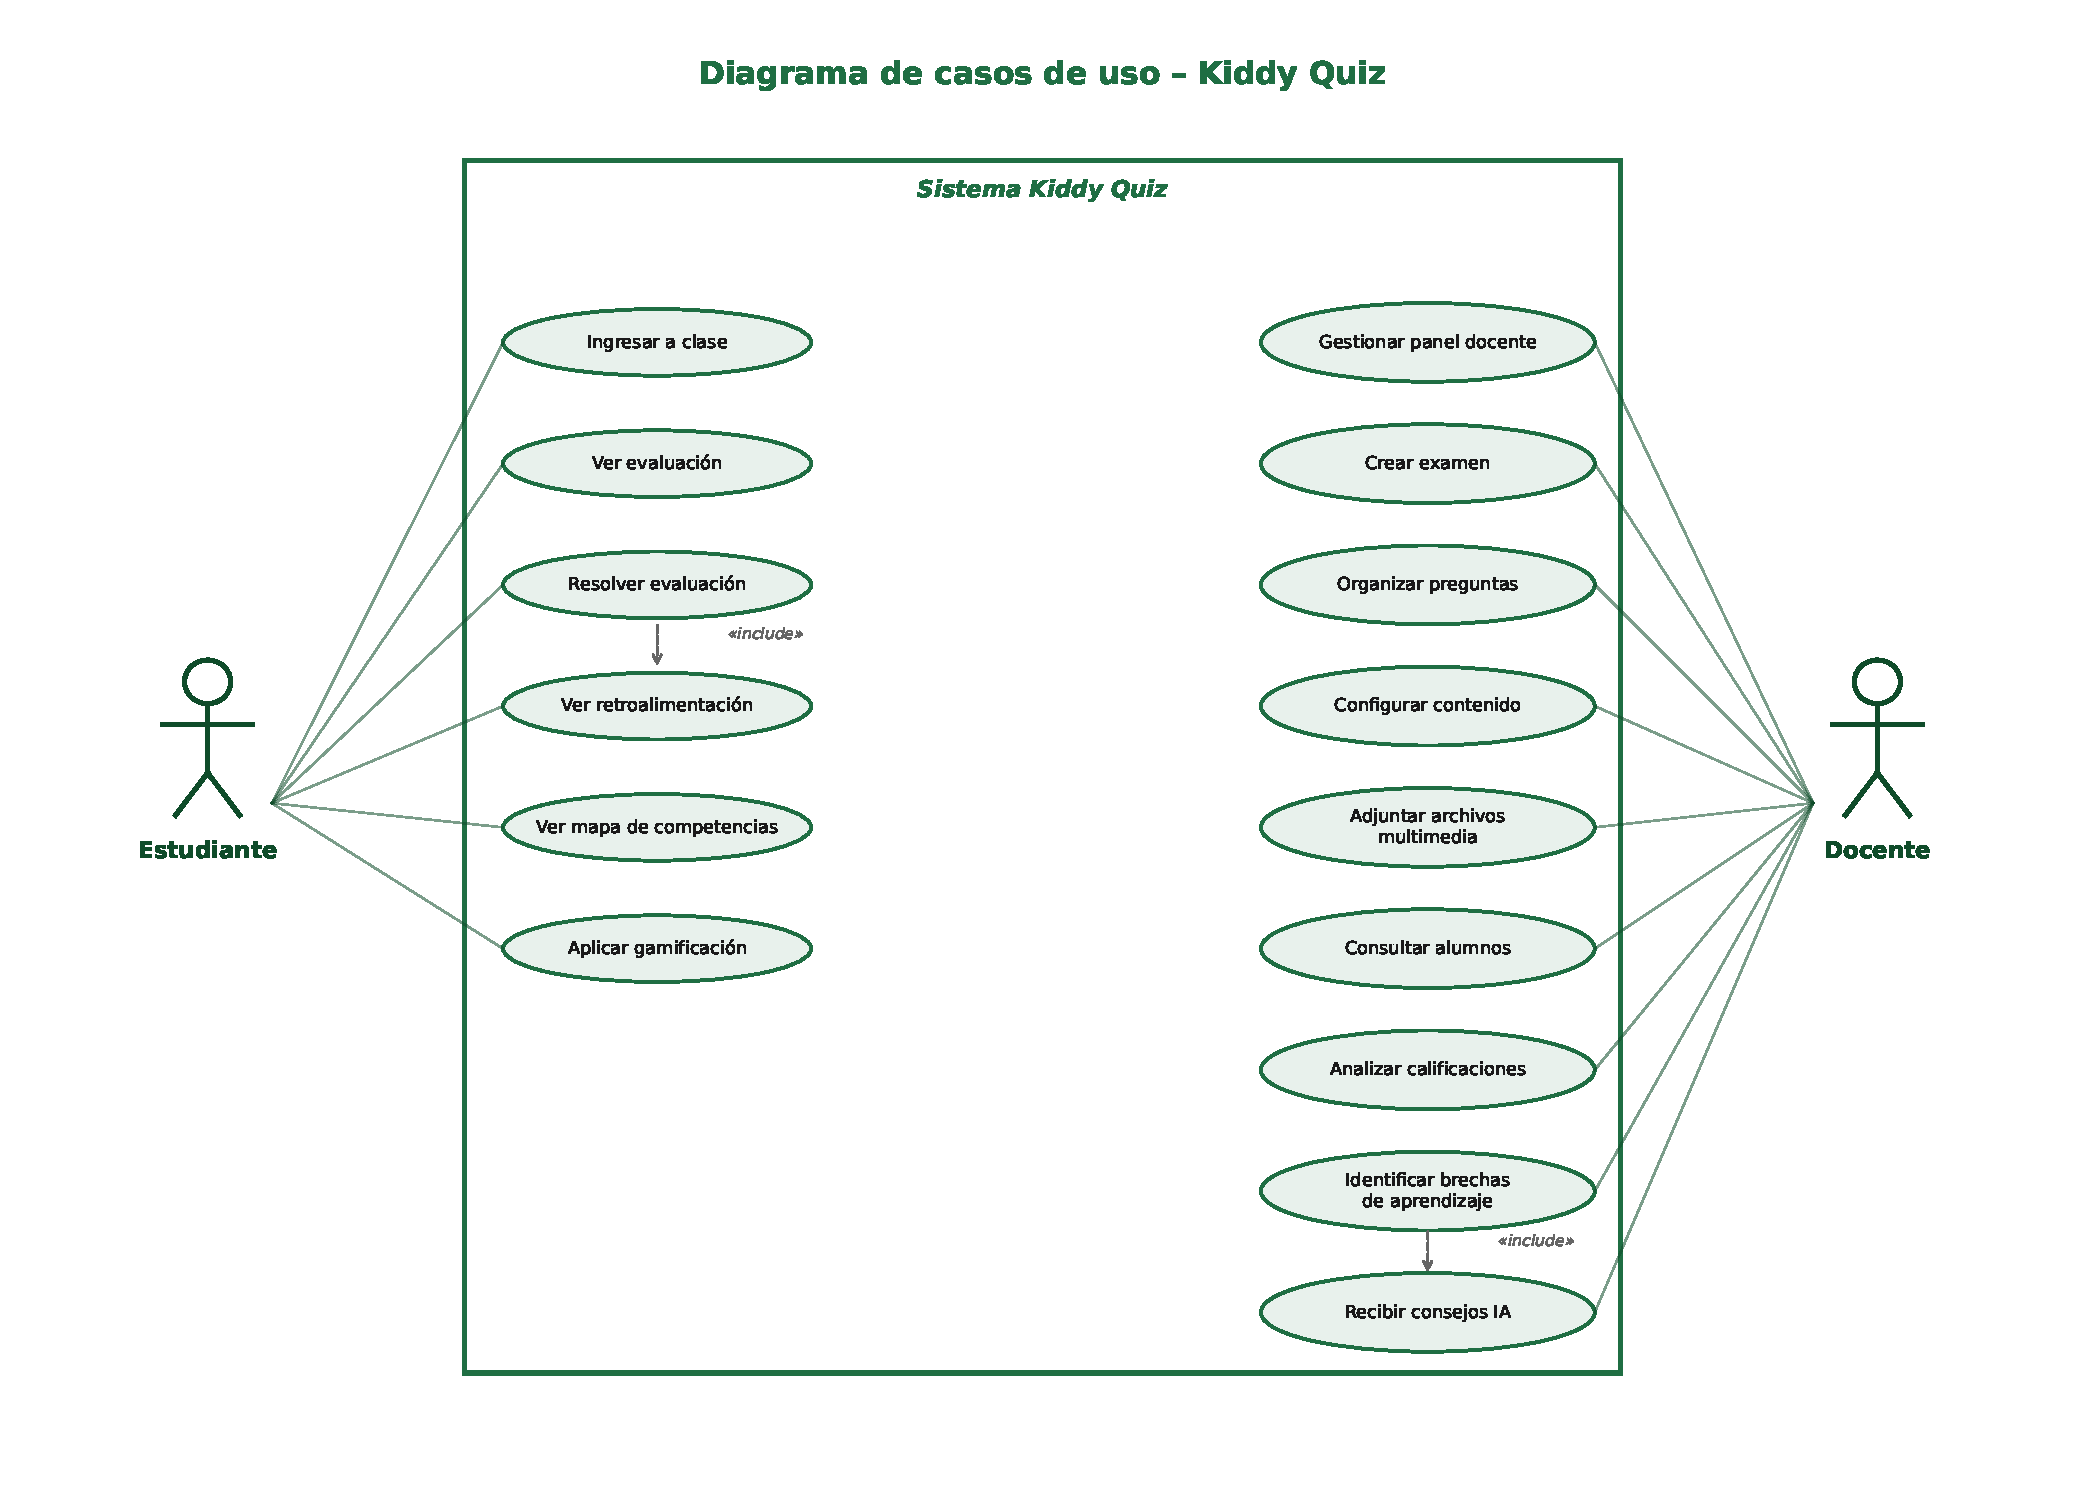
\includegraphics[width=\textwidth]{figuras/fig03_casos_uso.pdf}
\fuenteautor
\end{figure}

El estudiante interactúa con la aplicación principalmente para visualizar las clases a las que pertenece, unirse a nuevas mediante un código de acceso y desarrollar las evaluaciones estructuradas por el docente. Adicionalmente, este perfil le permite consultar los detalles de sus resultados, monitorear su progreso académico general y acceder a la retroalimentación motivacional generada por la inteligencia artificial. Por su parte, las interacciones principales del docente consisten en la administración integral del entorno académico: el profesor utiliza el sistema para crear y gestionar clases, administrar el listado de estudiantes y emplear un editor completo para la creación de evaluaciones. Los casos de uso seleccionados se han elegido por su alta relevancia y alineación directa con los objetivos del proyecto.

\subsection{Descripción de los casos de uso extendidos}

A continuación se especifican los casos de uso derivados de la Ilustración~\ref{fig:casos_uso}. Para ello, se han seleccionado las interacciones más significativas del sistema, haciendo especial énfasis en las funcionalidades relacionadas con la evaluación por competencias.

\begin{table}[H]
\centering
\caption{Caso de uso ``Ver evaluación''.}
\label{tab:cu_ver_eval}
\begin{small}
\begin{tabularx}{\textwidth}{|L{3cm}|X|}
\hline
\rowcolor{tabhead}
\tabhead{Código:} CU-003 & \tabhead{Actor:} Estudiante\\
\hline
\textbf{Objetivo} & Permitir al estudiante visualizar de forma organizada y atractiva las pruebas que su docente ha habilitado para su resolución.\\
\hline
\textbf{Resumen} & Al ingresar al sistema, el estudiante observa una cuadrícula de tarjetas que representan las evaluaciones activas, lo que le permite identificar temas y niveles de dificultad antes de comenzar.\\
\hline
\textbf{Tipo} & Principal\\
\hline
\textbf{Dependencias} & Invoca a CU-004 (Resolver evaluación). Depende de la base de datos de evaluaciones y filtros por estado.\\
\hline
\textbf{Precondición} & El estudiante debe estar autenticado y vinculado a un docente; debe existir al menos una evaluación habilitada.\\
\hline
\textbf{Postcondición} & El estudiante visualiza las tarjetas en pantalla y el sistema queda a la espera de la selección.\\
\hline
\textbf{Flujo normal} & 1.~Inicio de sesión exitoso. 2.~El sistema consulta evaluaciones vinculadas. 3.~Filtra por estado ``habilitada''. 4.~Renderiza cuadrícula. 5.~El estudiante selecciona una. 6.~Redirección a CU-004.\\
\hline
\textbf{Flujo alterno} & 3.a~Sin evaluaciones disponibles: el sistema muestra un mensaje amigable. 4.a~Error de carga multimedia: ícono temático por defecto.\\
\hline
\end{tabularx}
\end{small}
\fuenteautor
\end{table}

\begin{table}[H]
\centering
\caption{Caso de uso ``Resolver evaluación''.}
\label{tab:cu_resolver}
\begin{small}
\begin{tabularx}{\textwidth}{|L{3cm}|X|}
\hline
\rowcolor{tabhead}
\tabhead{Código:} CU-004 & \tabhead{Actor:} Estudiante\\
\hline
\textbf{Objetivo} & Proporcionar un entorno interactivo y amigable para que el estudiante responda las preguntas de una evaluación de forma secuencial.\\
\hline
\textbf{Resumen} & El estudiante accede a la prueba, lee las instrucciones y responde los ítems uno a uno. El sistema permite navegación asistida y guarda el progreso automáticamente.\\
\hline
\textbf{Tipo} & Principal\\
\hline
\textbf{Dependencias} & Invoca a CU-005 (Ver retroalimentación). Depende del motor de evaluación y de la base de datos de preguntas.\\
\hline
\textbf{Precondición} & El estudiante debe haber seleccionado una evaluación válida desde su panel (CU-003).\\
\hline
\textbf{Postcondición} & El sistema captura todas las respuestas y las envía al \textit{backend} para su cálculo.\\
\hline
\textbf{Flujo normal} & 1.~Despliegue de la primera pregunta. 2.~El estudiante selecciona o introduce su respuesta. 3.~Validación cliente. 4.~Avance a la siguiente pregunta. 5.~Al finalizar, envío al servidor. 6.~Cálculo del puntaje.\\
\hline
\textbf{Flujo alterno} & 2.a~Tiempo agotado: cierre automático y envío de respuestas registradas. 5.a~Pérdida de conexión: persistencia local mediante \textit{LocalStorage}.\\
\hline
\end{tabularx}
\end{small}
\fuenteautor
\end{table}

\begin{table}[H]
\centering
\caption{Caso de uso ``Ver retroalimentación''.}
\label{tab:cu_retro}
\begin{small}
\begin{tabularx}{\textwidth}{|L{3cm}|X|}
\hline
\rowcolor{tabhead}
\tabhead{Código:} CU-005 & \tabhead{Actor:} Estudiante\\
\hline
\textbf{Objetivo} & Mostrar al estudiante un reporte motivacional generado por IA, con su puntaje y consejos personalizados.\\
\hline
\textbf{Resumen} & Tras finalizar la prueba, el sistema invoca a Gemini AI para generar un mensaje personalizado y muestra los resultados en formato amigable.\\
\hline
\textbf{Tipo} & Principal\\
\hline
\textbf{Dependencias} & Invocado por CU-004. Requiere conexión a la API de Gemini.\\
\hline
\textbf{Flujo normal} & 1.~Recepción del puntaje. 2.~Construcción de \textit{prompt}. 3.~Llamada a Gemini API. 4.~Renderizado del mensaje y gráficos.\\
\hline
\textbf{Flujo alterno} & 3.a~Falla de la API: se muestra un mensaje motivacional genérico.\\
\hline
\end{tabularx}
\end{small}
\fuenteautor
\end{table}

\begin{table}[H]
\centering
\caption{Caso de uso ``Gestionar panel docente''.}
\label{tab:cu_panel}
\begin{small}
\begin{tabularx}{\textwidth}{|L{3cm}|X|}
\hline
\rowcolor{tabhead}
\tabhead{Código:} CU-006 & \tabhead{Actor:} Docente\\
\hline
\textbf{Objetivo} & Centralizar la gestión académica del docente: clases, evaluaciones y estudiantes.\\
\hline
\textbf{Resumen} & El docente accede a un panel con accesos rápidos para crear, editar y monitorear sus clases y evaluaciones.\\
\hline
\textbf{Flujo normal} & 1.~Inicio de sesión como docente. 2.~Redirección al panel. 3.~Visualización de clases activas. 4.~Selección de una acción (crear clase, gestionar estudiantes, etc.).\\
\hline
\end{tabularx}
\end{small}
\fuenteautor
\end{table}

\begin{table}[H]
\centering
\caption{Caso de uso ``Crear examen''.}
\label{tab:cu_crear_examen}
\begin{small}
\begin{tabularx}{\textwidth}{|L{3cm}|X|}
\hline
\rowcolor{tabhead}
\tabhead{Código:} CU-007 & \tabhead{Actor:} Docente\\
\hline
\textbf{Objetivo} & Permitir al docente diseñar una nueva evaluación con título, descripción, dificultad y duración.\\
\hline
\textbf{Flujo normal} & 1.~Selección de ``crear examen'' en el panel. 2.~Llenado del formulario base. 3.~Adición de preguntas (CU-008). 4.~Guardado y publicación opcional.\\
\hline
\end{tabularx}
\end{small}
\fuenteautor
\end{table}

\begin{table}[H]
\centering
\caption{Caso de uso ``Organizar preguntas''.}
\label{tab:cu_org_preg}
\begin{small}
\begin{tabularx}{\textwidth}{|L{3cm}|X|}
\hline
\rowcolor{tabhead}
\tabhead{Código:} CU-008 & \tabhead{Actor:} Docente\\
\hline
\textbf{Objetivo} & Permitir al docente añadir, editar, eliminar y reordenar las preguntas de un examen.\\
\hline
\textbf{Flujo normal} & 1.~Selección de la pestaña ``preguntas''. 2.~Operaciones CRUD mediante \textit{Drag \& Drop}. 3.~Guardado automático.\\
\hline
\end{tabularx}
\end{small}
\fuenteautor
\end{table}

\begin{table}[H]
\centering
\caption{Caso de uso ``Configurar contenido''.}
\label{tab:cu_config}
\begin{small}
\begin{tabularx}{\textwidth}{|L{3cm}|X|}
\hline
\rowcolor{tabhead}
\tabhead{Código:} CU-009 & \tabhead{Actor:} Docente\\
\hline
\textbf{Objetivo} & Definir el tipo de pregunta (opción múltiple, unir columnas, secuencias, abierta) y sus opciones.\\
\hline
\textbf{Flujo normal} & 1.~Selección del tipo de pregunta. 2.~Configuración de opciones y respuesta correcta. 3.~Validación. 4.~Guardado.\\
\hline
\end{tabularx}
\end{small}
\fuenteautor
\end{table}

\begin{table}[H]
\centering
\caption{Caso de uso ``Adjuntar archivos multimedia''.}
\label{tab:cu_multimedia}
\begin{small}
\begin{tabularx}{\textwidth}{|L{3cm}|X|}
\hline
\rowcolor{tabhead}
\tabhead{Código:} CU-010 & \tabhead{Actor:} Docente\\
\hline
\textbf{Objetivo} & Adjuntar imágenes, GIFs o videos a las preguntas para potenciar el aprendizaje visual.\\
\hline
\textbf{Flujo normal} & 1.~Selección del botón ``adjuntar''. 2.~Carga del archivo a Cloudinary. 3.~Recepción de URL. 4.~Asociación a la pregunta.\\
\hline
\end{tabularx}
\end{small}
\fuenteautor
\end{table}

\begin{table}[H]
\centering
\caption{Caso de uso ``Consultar alumnos''.}
\label{tab:cu_alumnos}
\begin{small}
\begin{tabularx}{\textwidth}{|L{3cm}|X|}
\hline
\rowcolor{tabhead}
\tabhead{Código:} CU-011 & \tabhead{Actor:} Docente\\
\hline
\textbf{Objetivo} & Mostrar la lista de estudiantes inscritos en una clase y permitir filtrar por nombre o estado.\\
\hline
\textbf{Flujo normal} & 1.~Acceso a la pestaña ``alumnos''. 2.~Renderizado de la lista. 3.~Aplicación de filtros. 4.~Selección de un alumno para ver su detalle.\\
\hline
\end{tabularx}
\end{small}
\fuenteautor
\end{table}

\begin{table}[H]
\centering
\caption{Caso de uso ``Analizar calificaciones''.}
\label{tab:cu_analizar}
\begin{small}
\begin{tabularx}{\textwidth}{|L{3cm}|X|}
\hline
\rowcolor{tabhead}
\tabhead{Código:} CU-012 & \tabhead{Actor:} Docente\\
\hline
\textbf{Objetivo} & Mostrar al docente el promedio global y el desglose por evaluación de cada estudiante.\\
\hline
\textbf{Flujo normal} & 1.~Selección de un alumno. 2.~Consulta de su historial. 3.~Cálculo de estadísticas. 4.~Renderizado de gráficos.\\
\hline
\end{tabularx}
\end{small}
\fuenteautor
\end{table}

\begin{table}[H]
\centering
\caption{Caso de uso ``Identificar brechas de aprendizaje''.}
\label{tab:cu_brechas}
\begin{small}
\begin{tabularx}{\textwidth}{|L{3cm}|X|}
\hline
\rowcolor{tabhead}
\tabhead{Código:} CU-013 & \tabhead{Actor:} Docente\\
\hline
\textbf{Objetivo} & Detectar áreas temáticas con bajo rendimiento mediante análisis por categoría.\\
\hline
\textbf{Flujo normal} & 1.~Cálculo de aciertos por categoría. 2.~Identificación de categorías por debajo del umbral. 3.~Renderizado de visualización destacada.\\
\hline
\end{tabularx}
\end{small}
\fuenteautor
\end{table}

\begin{table}[H]
\centering
\caption{Caso de uso ``Recibir consejos IA''.}
\label{tab:cu_consejos}
\begin{small}
\begin{tabularx}{\textwidth}{|L{3cm}|X|}
\hline
\rowcolor{tabhead}
\tabhead{Código:} CU-014 & \tabhead{Actor:} Docente / Estudiante\\
\hline
\textbf{Objetivo} & Generar sugerencias pedagógicas basadas en patrones de error mediante Gemini AI.\\
\hline
\textbf{Flujo normal} & 1.~Análisis del histórico. 2.~Construcción de \textit{prompt} con contexto. 3.~Invocación al modelo. 4.~Presentación del consejo.\\
\hline
\end{tabularx}
\end{small}
\fuenteautor
\end{table}

\begin{table}[H]
\centering
\caption{Caso de uso ``Aplicar gamificación''.}
\label{tab:cu_gamificacion}
\begin{small}
\begin{tabularx}{\textwidth}{|L{3cm}|X|}
\hline
\rowcolor{tabhead}
\tabhead{Código:} CU-015 & \tabhead{Actor:} Estudiante\\
\hline
\textbf{Objetivo} & Aplicar mecánicas de juego (insignias, niveles, recompensas) durante la resolución de evaluaciones.\\
\hline
\textbf{Flujo normal} & 1.~Selección del modo lúdico. 2.~Asignación de avatar. 3.~Despliegue de la prueba con elementos animados. 4.~Otorgamiento de insignias al finalizar.\\
\hline
\end{tabularx}
\end{small}
\fuenteautor
\end{table}

\begin{table}[H]
\centering
\caption{Caso de uso ``Ingresar a clase''.}
\label{tab:cu_ingresar}
\begin{small}
\begin{tabularx}{\textwidth}{|L{3cm}|X|}
\hline
\rowcolor{tabhead}
\tabhead{Código:} CU-016 & \tabhead{Actor:} Estudiante\\
\hline
\textbf{Objetivo} & Permitir al estudiante unirse a una clase mediante un código de acceso compartido por el docente.\\
\hline
\textbf{Flujo normal} & 1.~Acceso al panel del estudiante. 2.~Introducción del código de acceso. 3.~Validación. 4.~Inscripción automática.\\
\hline
\end{tabularx}
\end{small}
\fuenteautor
\end{table}

\begin{table}[H]
\centering
\caption{Caso de uso ``Ver mapa de competencias''.}
\label{tab:cu_mapa}
\begin{small}
\begin{tabularx}{\textwidth}{|L{3cm}|X|}
\hline
\rowcolor{tabhead}
\tabhead{Código:} CU-017 & \tabhead{Actor:} Docente / Estudiante\\
\hline
\textbf{Objetivo} & Visualizar el progreso por competencias mediante una representación gráfica en cuadros y colores.\\
\hline
\textbf{Resumen} & El sistema despliega una lista de competencias por módulo y nivel, indicando el estado (lograda, en proceso, no iniciada).\\
\hline
\textbf{Flujo normal} & 1.~Consulta del progreso. 2.~Recuperación del histórico. 3.~Cálculo del estado. 4.~Despliegue. 5.~Opción de exportar a PDF/Excel.\\
\hline
\textbf{Flujos alternos} & 2.a~Sin datos previos: todas las áreas figuran como ``no iniciada'' y se sugiere realizar una prueba diagnóstica.\\
\hline
\end{tabularx}
\end{small}
\fuenteautor
\end{table}

\subsection{Diagrama de arquitectura}

En la Ilustración~\ref{fig:arquitectura} se expone la arquitectura implementada en la aplicación web. Para su desarrollo se adoptó un modelo cliente-servidor con el propósito de establecer una clara separación de responsabilidades entre la interfaz de usuario (\textit{frontend}) y la lógica del sistema (\textit{backend}). Esta estructuración facilita la administración eficiente de los recursos y contribuye a ofrecer una experiencia de usuario optimizada.

\begin{figure}[H]
\centering
\caption{Diagrama de arquitectura del sistema Kiddy Quiz.}
\label{fig:arquitectura}
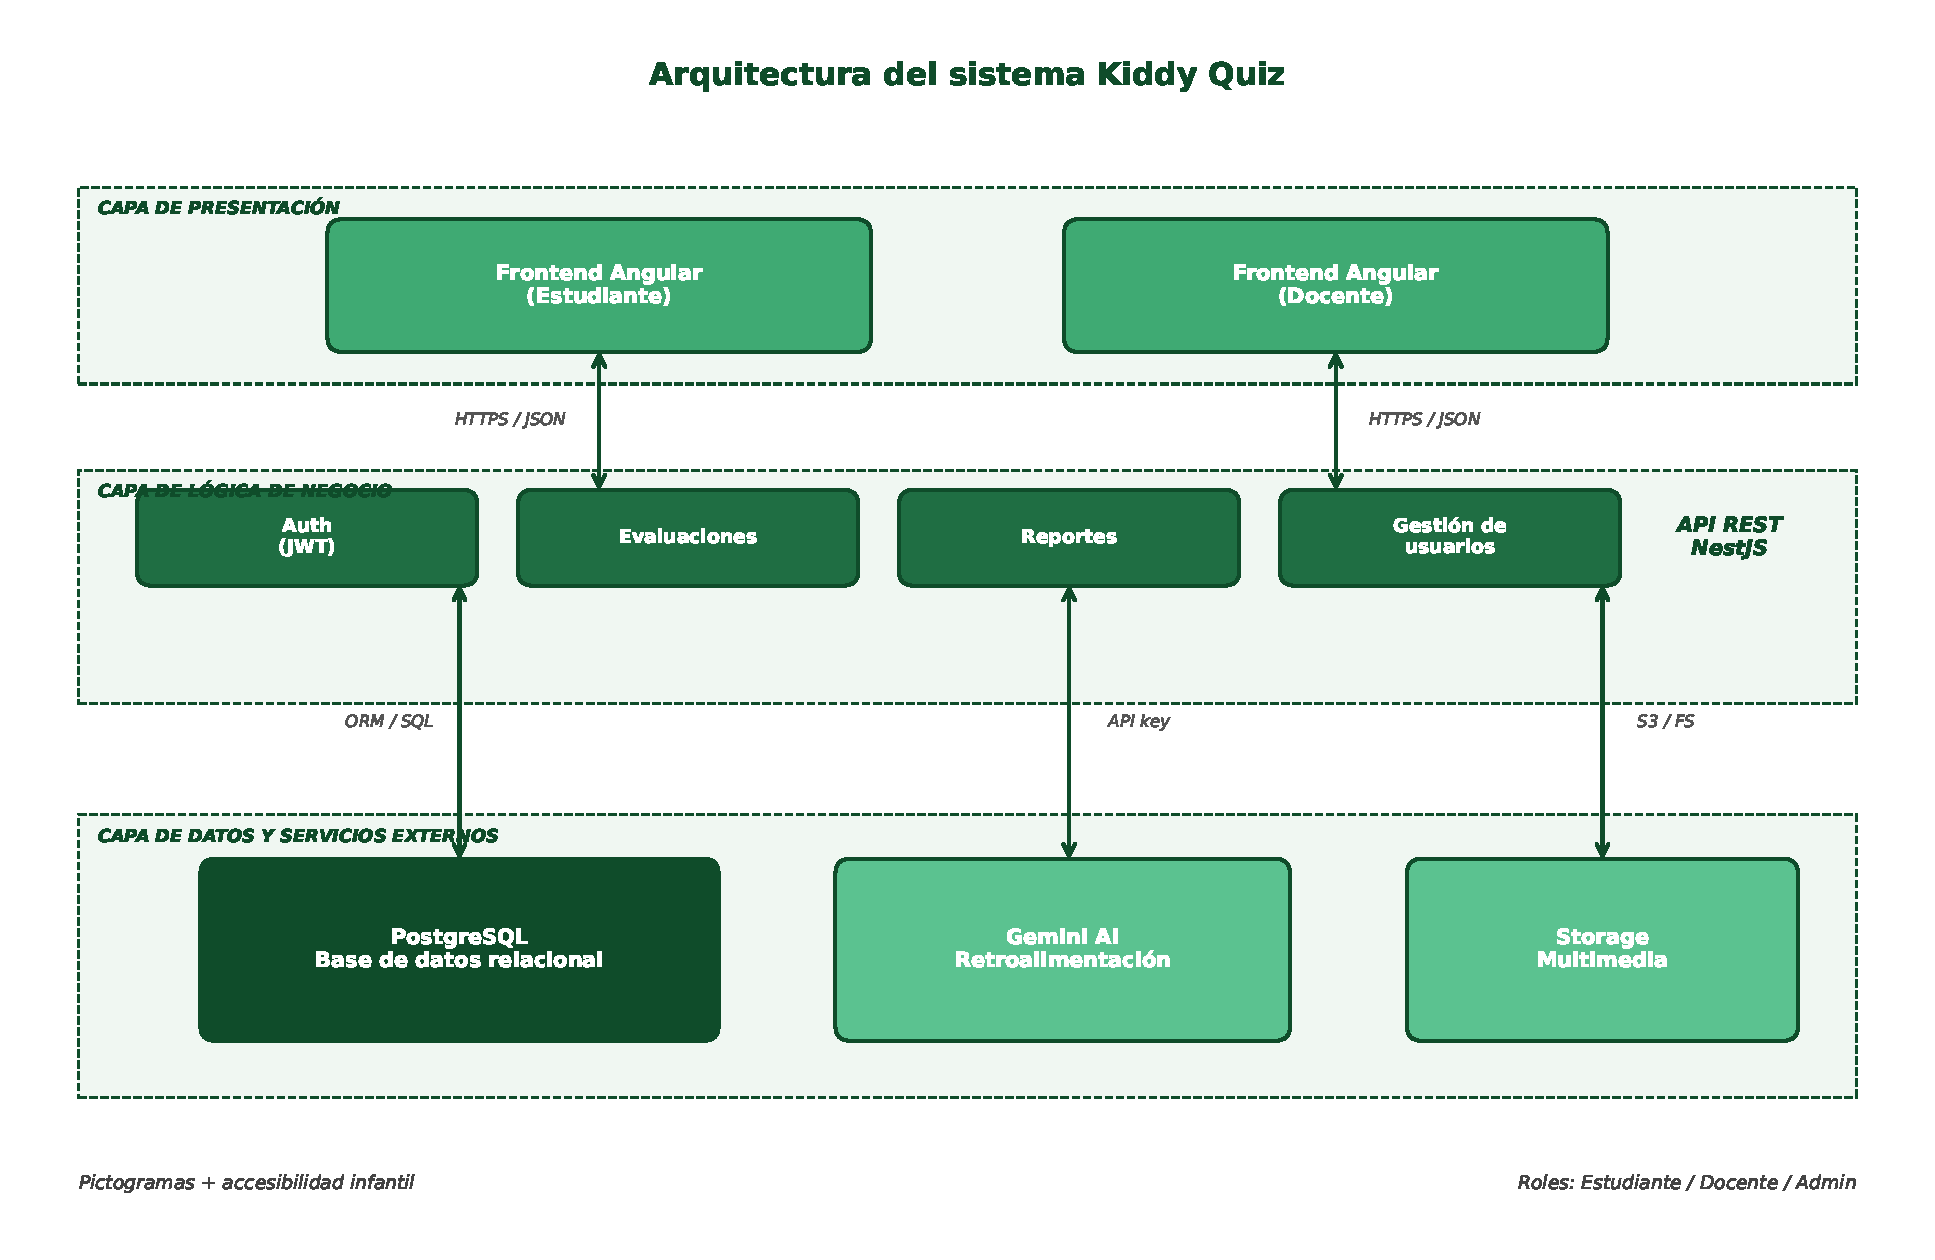
\includegraphics[width=\textwidth]{figuras/fig04_arquitectura.pdf}
\fuenteautor
\end{figure}

El \textit{frontend} de la aplicación, desarrollado mediante el \textit{framework} Angular, gestiona la interacción directa con los usuarios finales (estudiantes y docentes) y controla la presentación de las interfaces gráficas. Este componente se comunica con el servidor a través de peticiones API REST, intercambiando información en formato JSON. Por su parte, el \textit{backend}, implementado con NestJS, centraliza la lógica de negocio, la gestión de datos y los protocolos de seguridad y autenticación. A nivel de persistencia, el sistema emplea el motor de base de datos PostgreSQL, garantizando un almacenamiento estructurado, eficiente y escalable. Adicionalmente, la arquitectura se complementa con la integración de servicios externos clave: Gemini AI \cite{ref46_app_educativas}, utilizado para la generación de retroalimentación académica automatizada, y Cloudinary, empleado para el almacenamiento y la gestión optimizada de los recursos multimedia.

\subsection{Diagrama de base de datos}

En la Ilustración~\ref{fig:bd} se presenta el modelo físico de la base de datos, estructurado bajo un enfoque relacional. Cada tabla representa una entidad específica del sistema Kiddy Quiz, y sus relaciones se encuentran claramente definidas mediante claves foráneas, lo cual garantiza la integridad referencial y una correcta normalización de los datos.

\begin{figure}[H]
\centering
\caption{Modelo de base de datos del sistema Kiddy Quiz.}
\label{fig:bd}
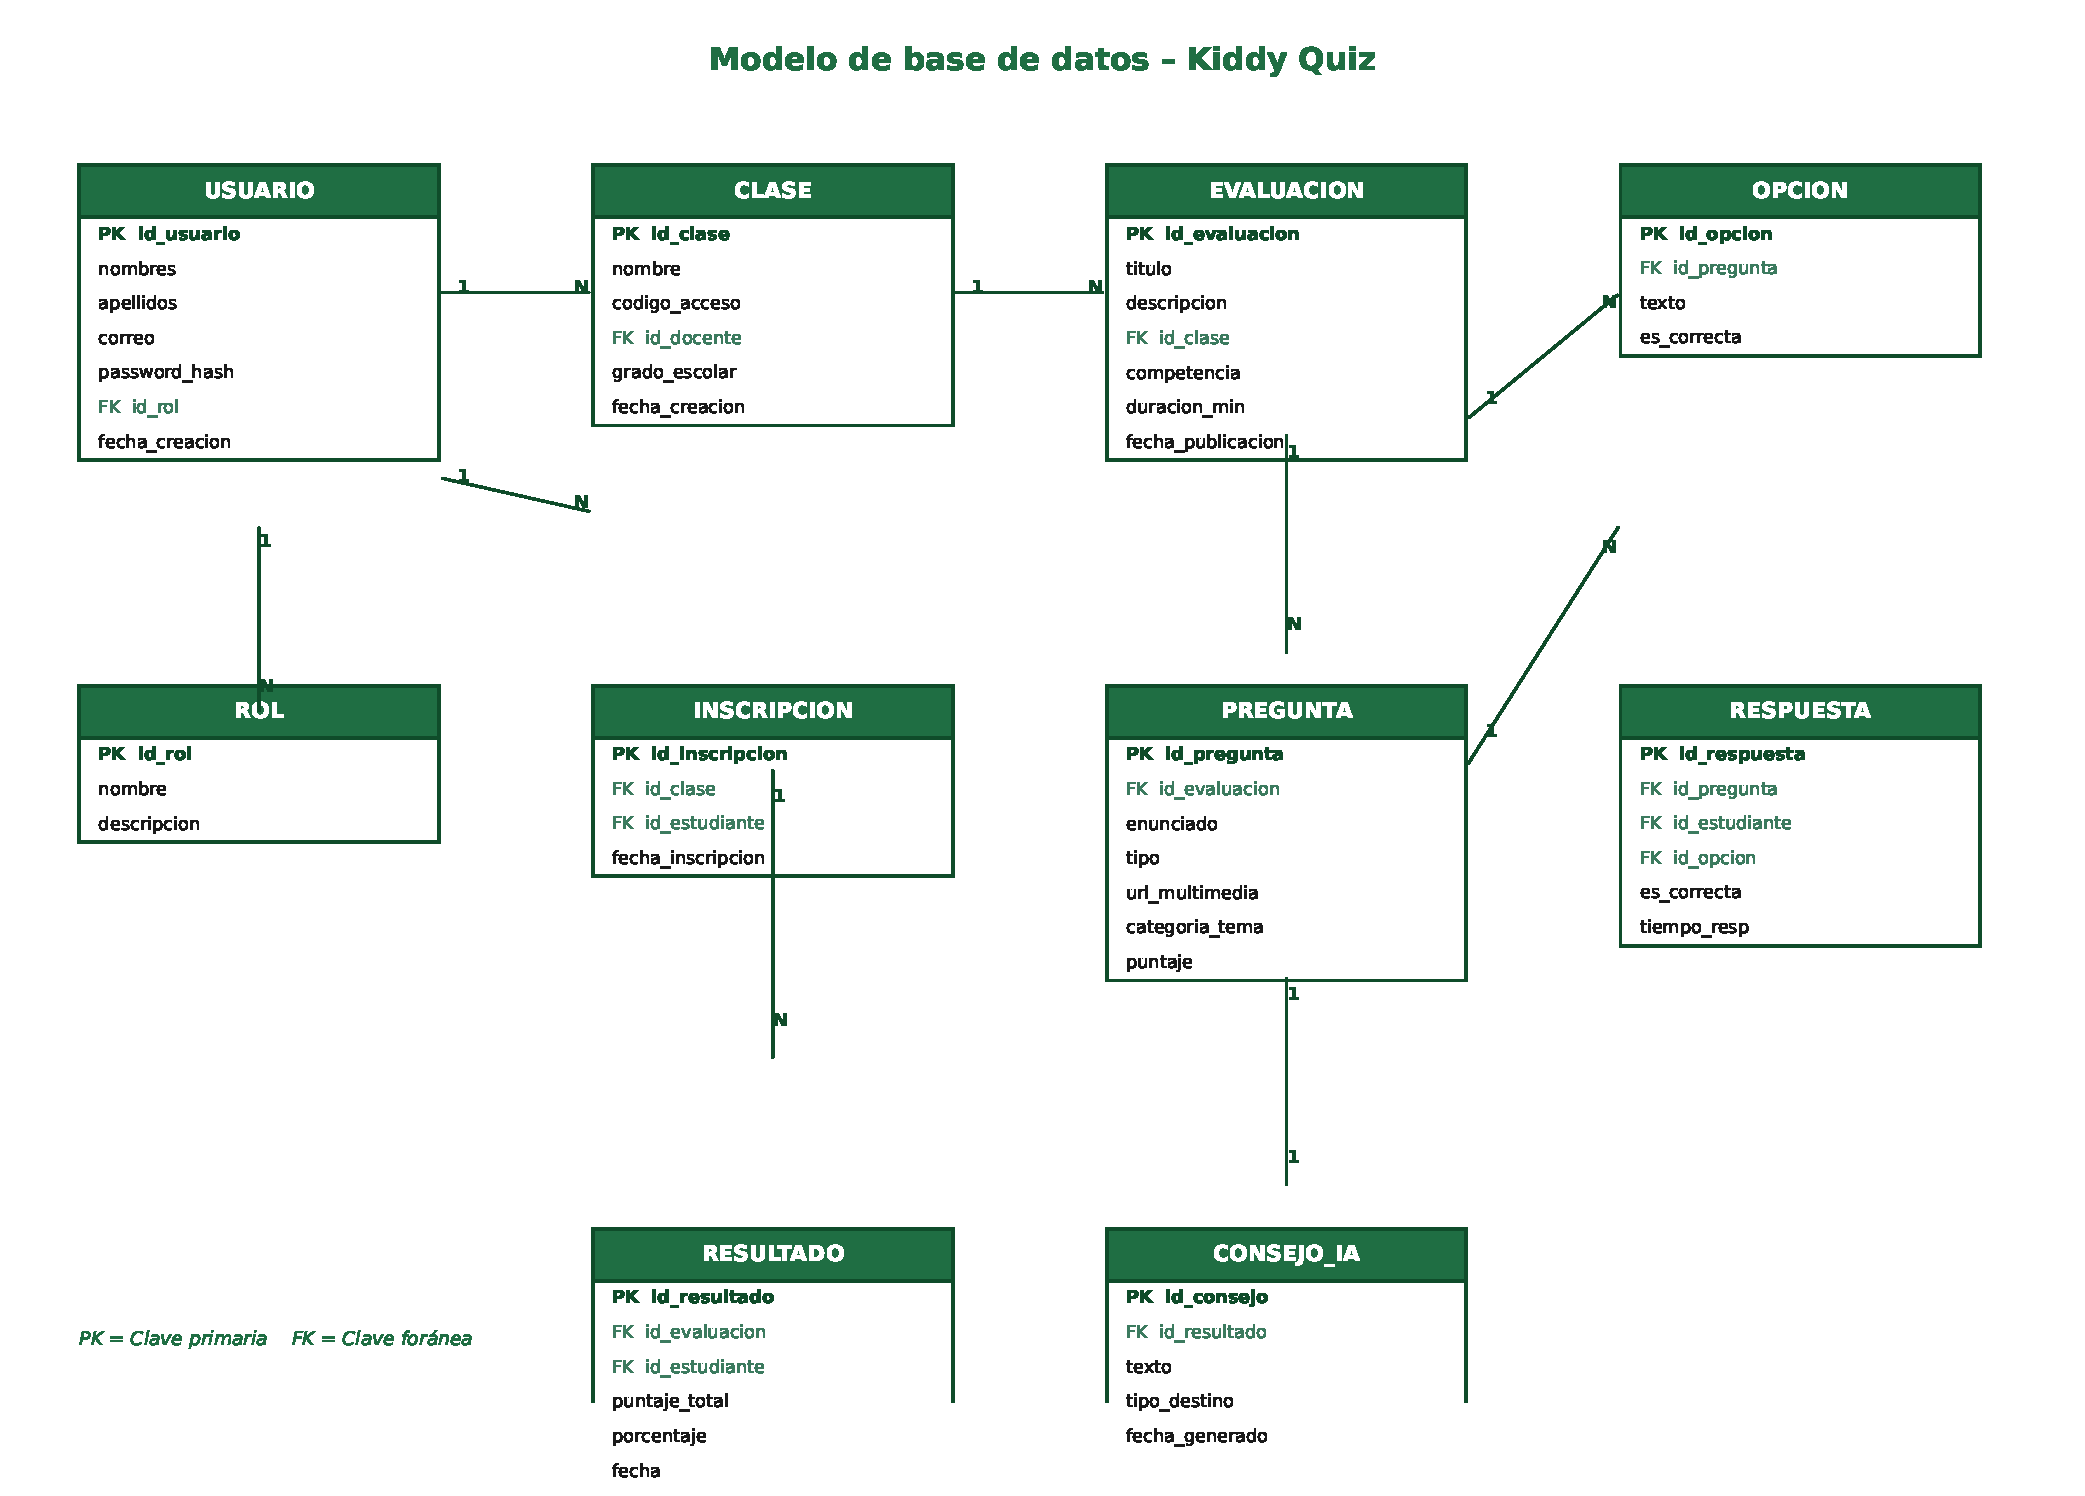
\includegraphics[width=\textwidth]{figuras/fig05_base_datos.pdf}
\fuenteautor
\end{figure}

En este esquema se destacan las interacciones centrales de la plataforma, tales como la gestión de usuarios (docentes y estudiantes), la administración de clases y la estructuración de las evaluaciones, las cuales se vinculan con sus respectivos bancos de preguntas y opciones. De igual manera, el diseño evidencia las entidades destinadas al registro continuo del desempeño académico, como el detalle de resolución y el progreso por competencias, información fundamental para la analítica del docente y el procesamiento de la IA. Implementada en PostgreSQL, esta estructura ha sido optimizada con los tipos de datos adecuados para asegurar la escalabilidad y el rendimiento de las consultas.

\subsection{Diseño del prototipo}

En este apartado se exponen los resultados correspondientes a la fase de diseño visual del sistema. Cabe destacar que, en congruencia con la metodología de Programación Extrema, el diseño no fue estático: durante la fase de entrevistas se utilizaron interfaces preliminares como base para recopilar la retroalimentación del docente experto. A partir de dichas observaciones y de las historias de usuario consolidadas, se iteró el diseño hasta llegar a los prototipos finales. En la Ilustración~\ref{fig:prototipo} se presenta el prototipo final maquetado en Figma, que resume el núcleo funcional, intuitivo y accesible de la plataforma.

\begin{figure}[H]
\centering
\caption{Prototipo final de la aplicación web Kiddy Quiz.}
\label{fig:prototipo}
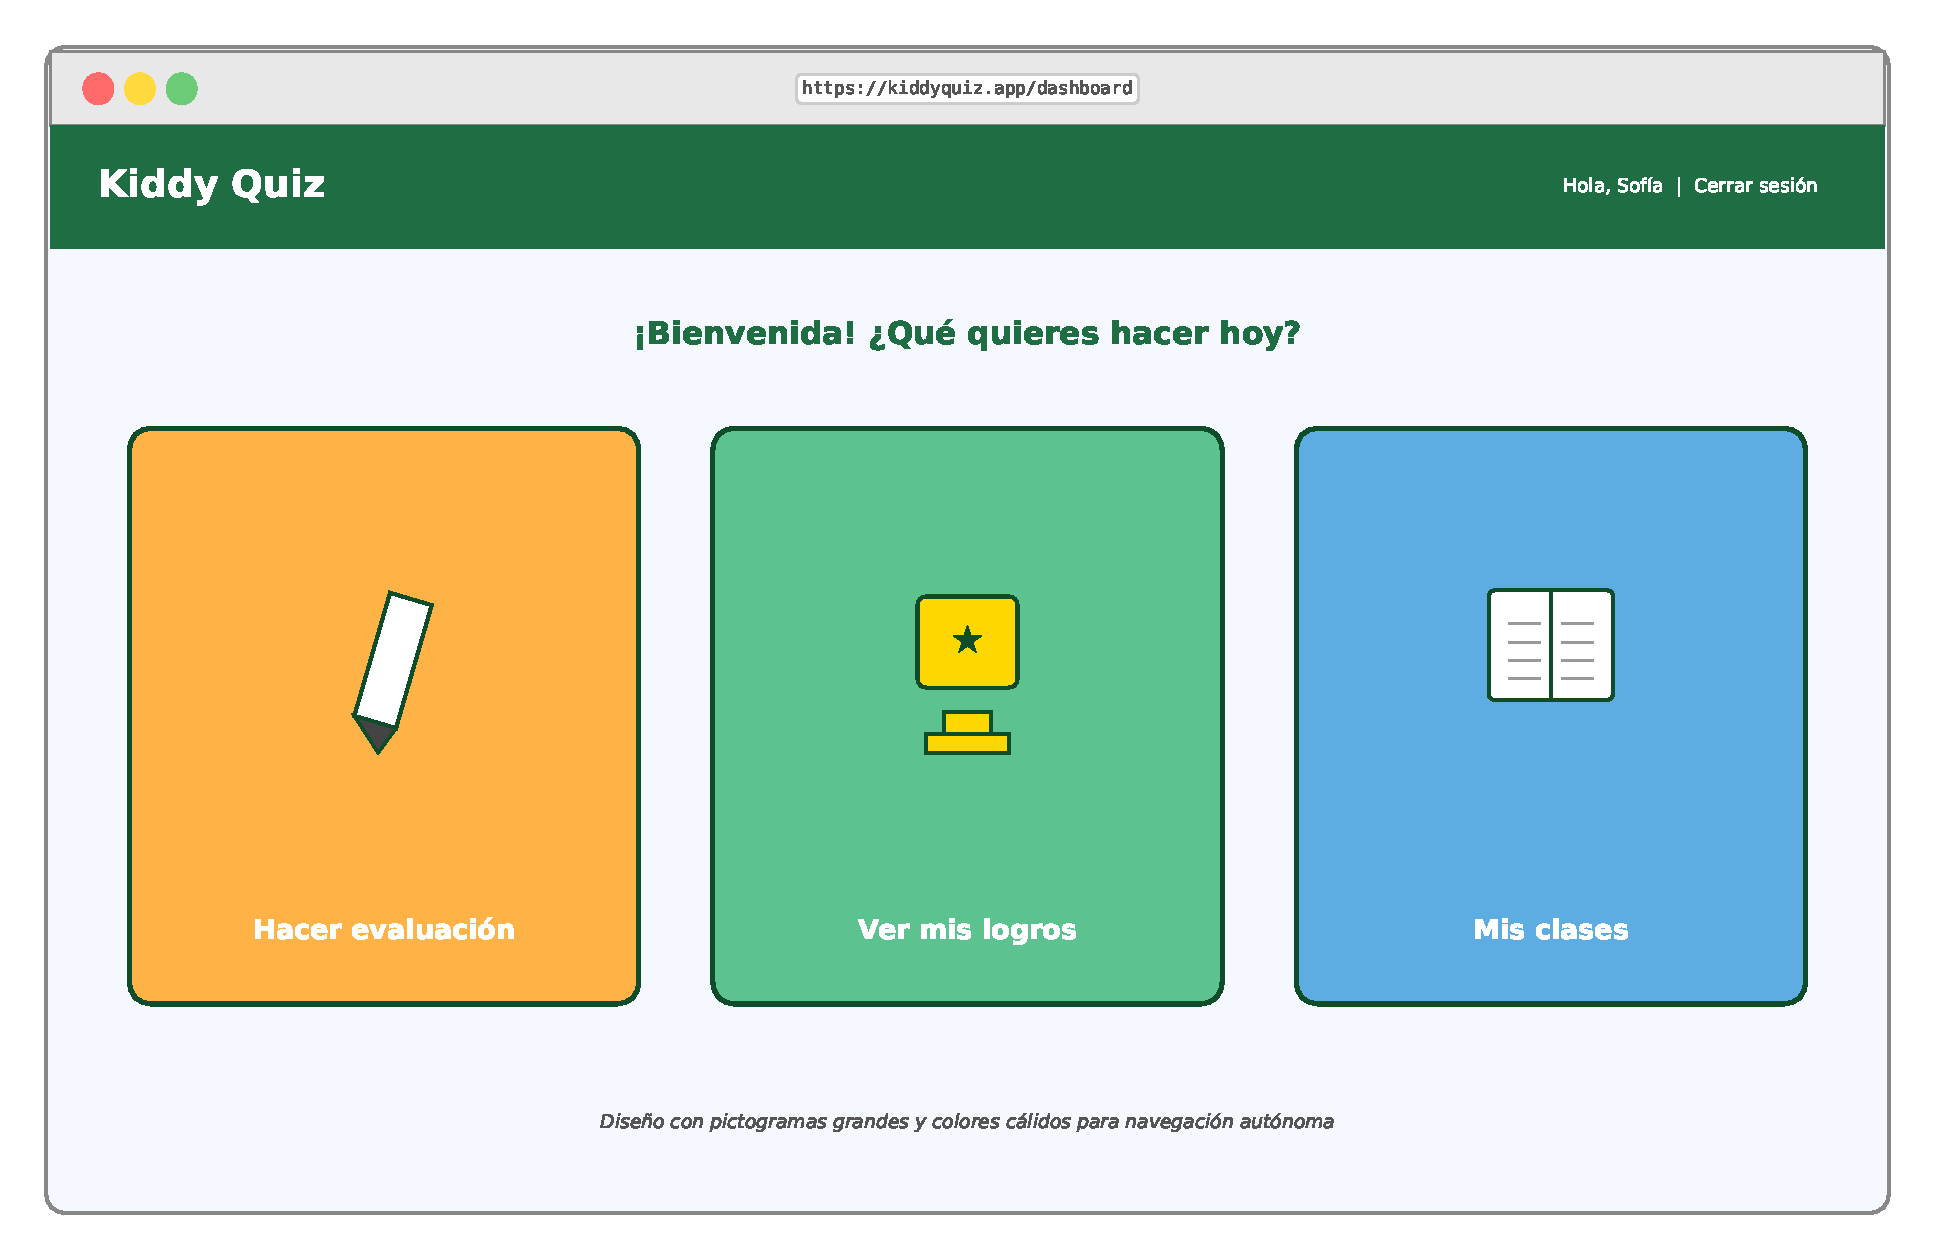
\includegraphics[width=\textwidth]{figuras/fig06_prototipo_final.pdf}
\fuenteautor
\end{figure}

A continuación, en la Ilustración~\ref{fig:modulo_eval} se visualiza el resultado funcional y estético del módulo destinado al estudiante durante la resolución de una evaluación. La captura evidencia una navegación simplificada, adaptada a las características de la educación básica elemental, y el uso de pictogramas como apoyo visual para los enunciados matemáticos.

\begin{figure}[H]
\centering
\caption{Módulo del estudiante: resolución de evaluación con pictogramas.}
\label{fig:modulo_eval}
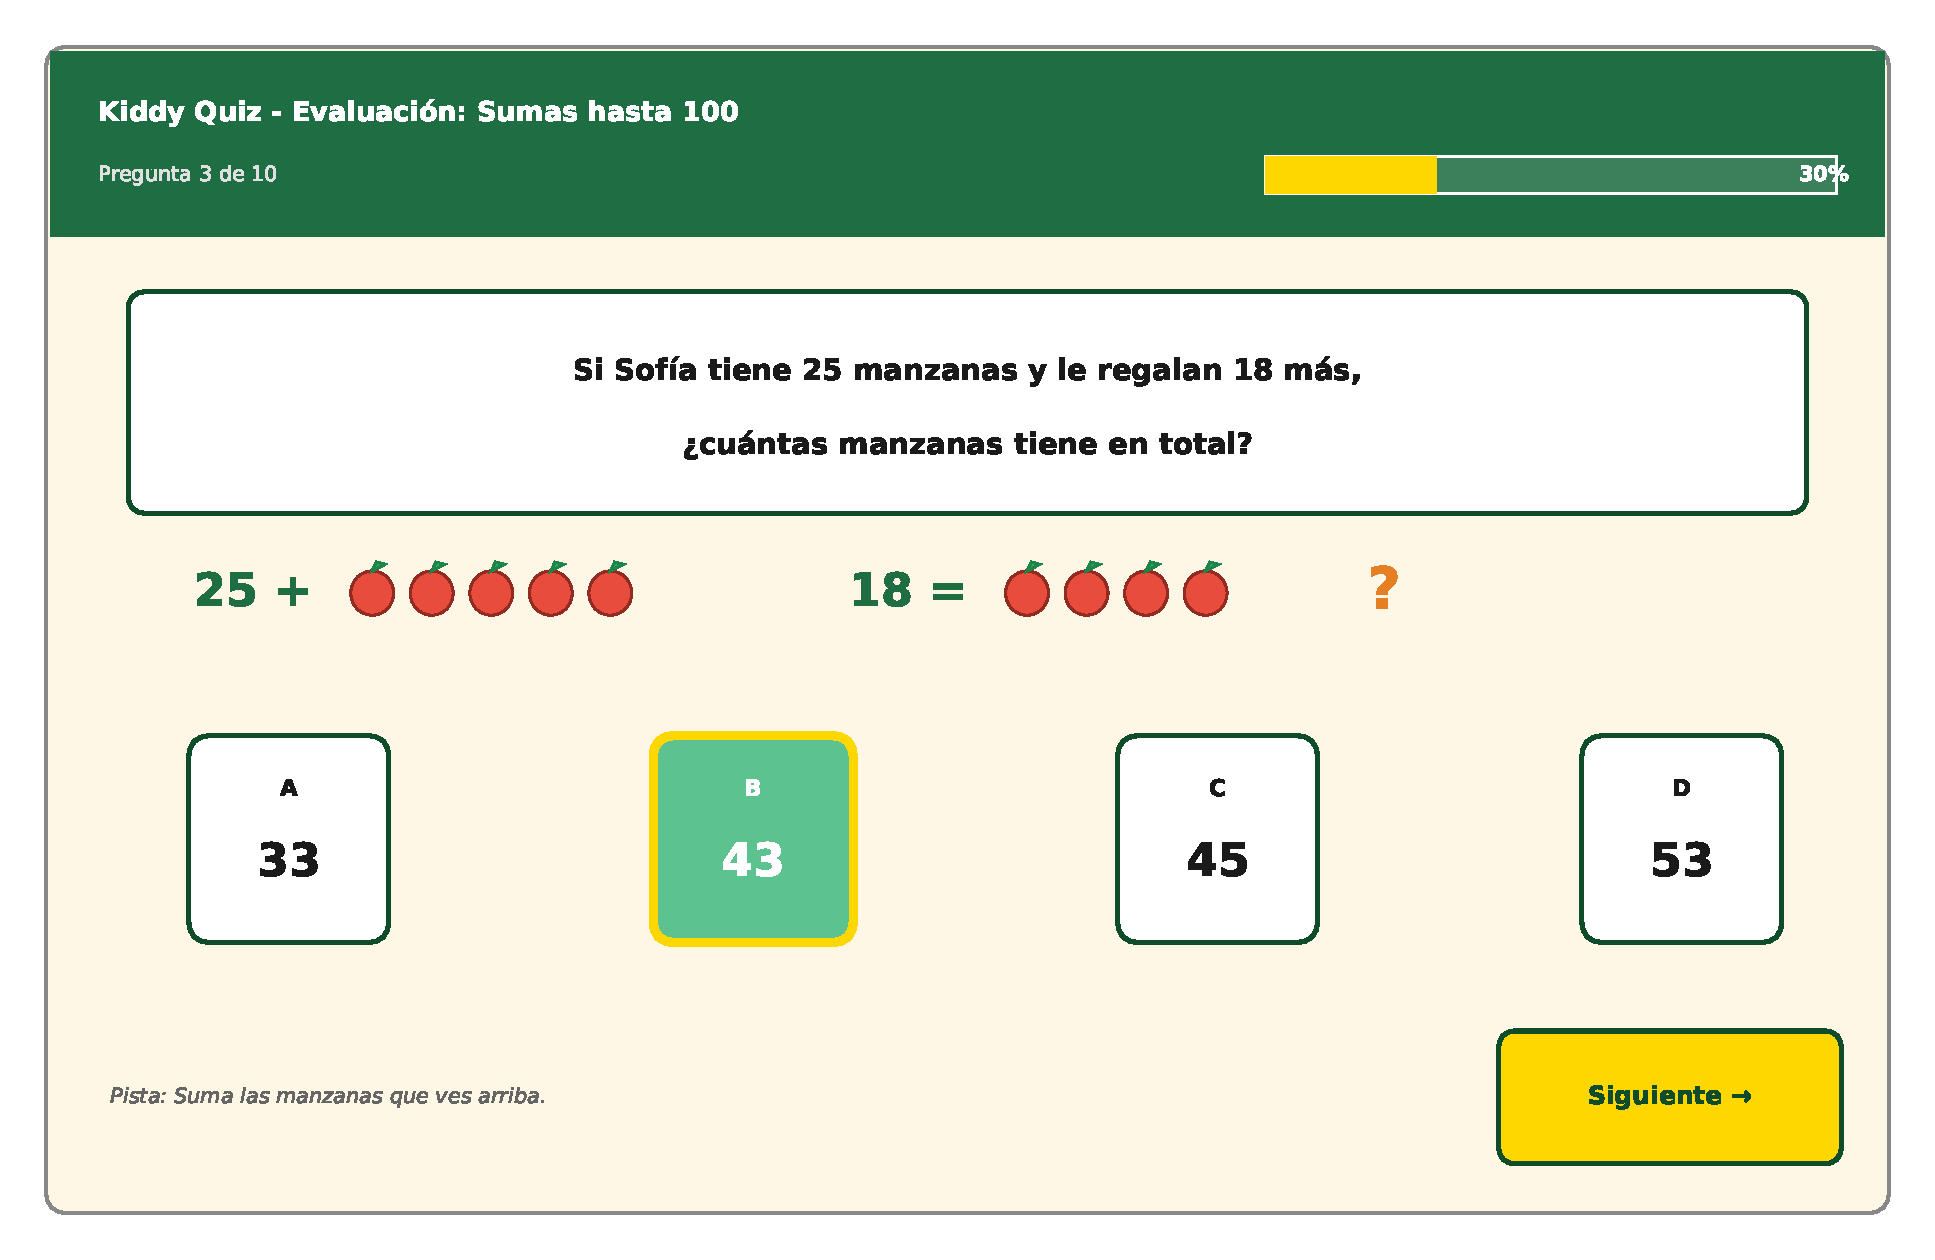
\includegraphics[width=\textwidth]{figuras/fig07_modulo_estudiante_eval.pdf}
\fuenteautor
\end{figure}

La Ilustración~\ref{fig:modulo_retro} presenta la pantalla de retroalimentación posterior a la evaluación, donde se materializa la integración de Gemini AI para ofrecer un acompañamiento continuo y motivacional al alumno. Se exhibe el puntaje obtenido, el desglose por áreas evaluadas y un mensaje generado por la IA que invita al estudiante a continuar practicando.

\begin{figure}[H]
\centering
\caption{Módulo del estudiante: pantalla de retroalimentación con feedback de Gemini AI.}
\label{fig:modulo_retro}
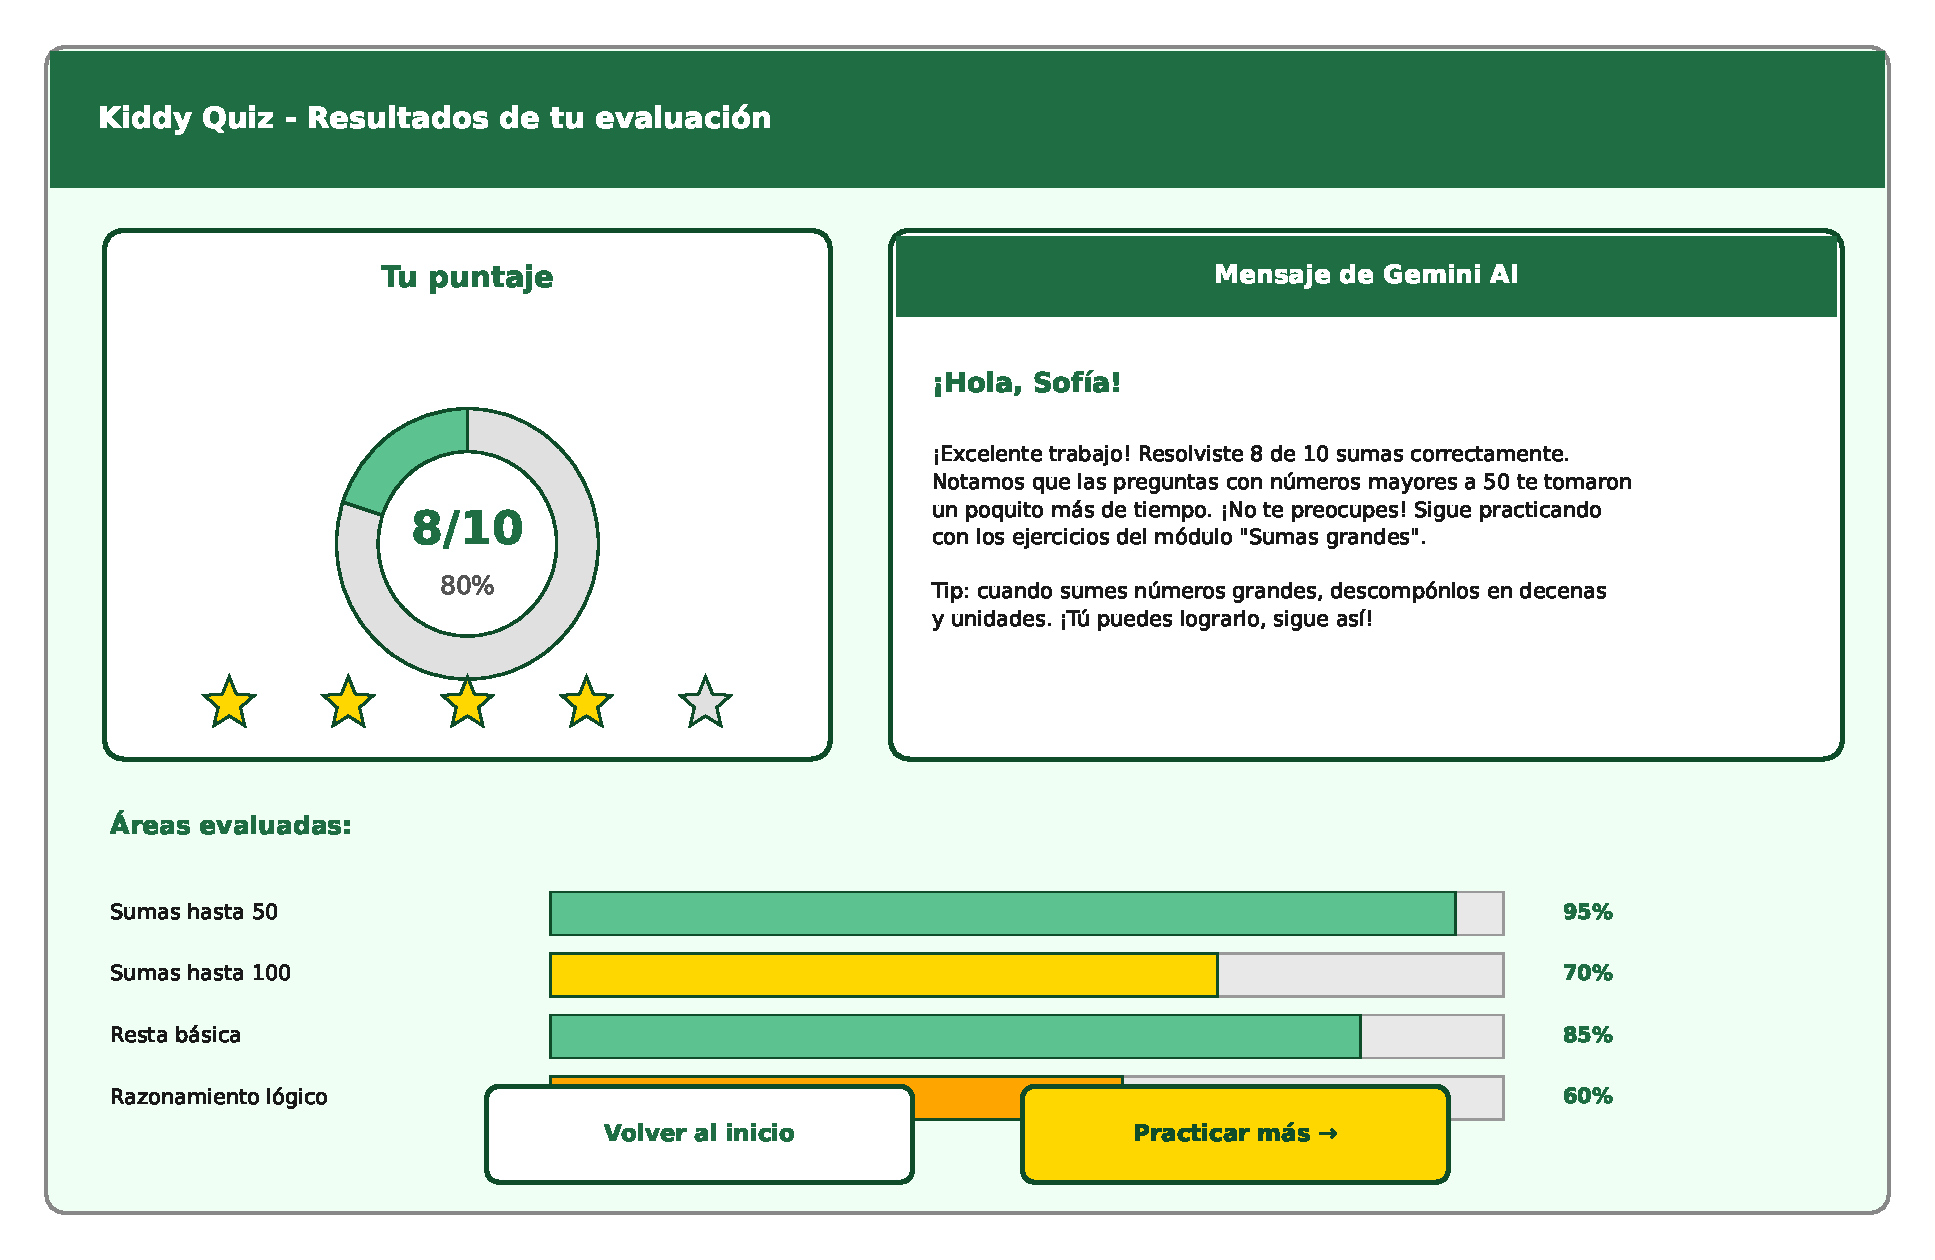
\includegraphics[width=\textwidth]{figuras/fig08_modulo_estudiante_retro.pdf}
\fuenteautor
\end{figure}

\subsection{Integración de Gemini AI}

La integración de la inteligencia artificial constituye uno de los ejes de mayor innovación tecnológica dentro del proyecto Kiddy Quiz. Para evidenciar esta implementación, en la Ilustración~\ref{fig:gemini} se expone un fragmento del código fuente correspondiente al servicio encargado de gestionar la comunicación con dicho modelo generativo desde el \textit{backend} estructurado en NestJS.

\begin{figure}[H]
\centering
\caption{Extracto del código de integración con Gemini AI en el \textit{backend} NestJS.}
\label{fig:gemini}
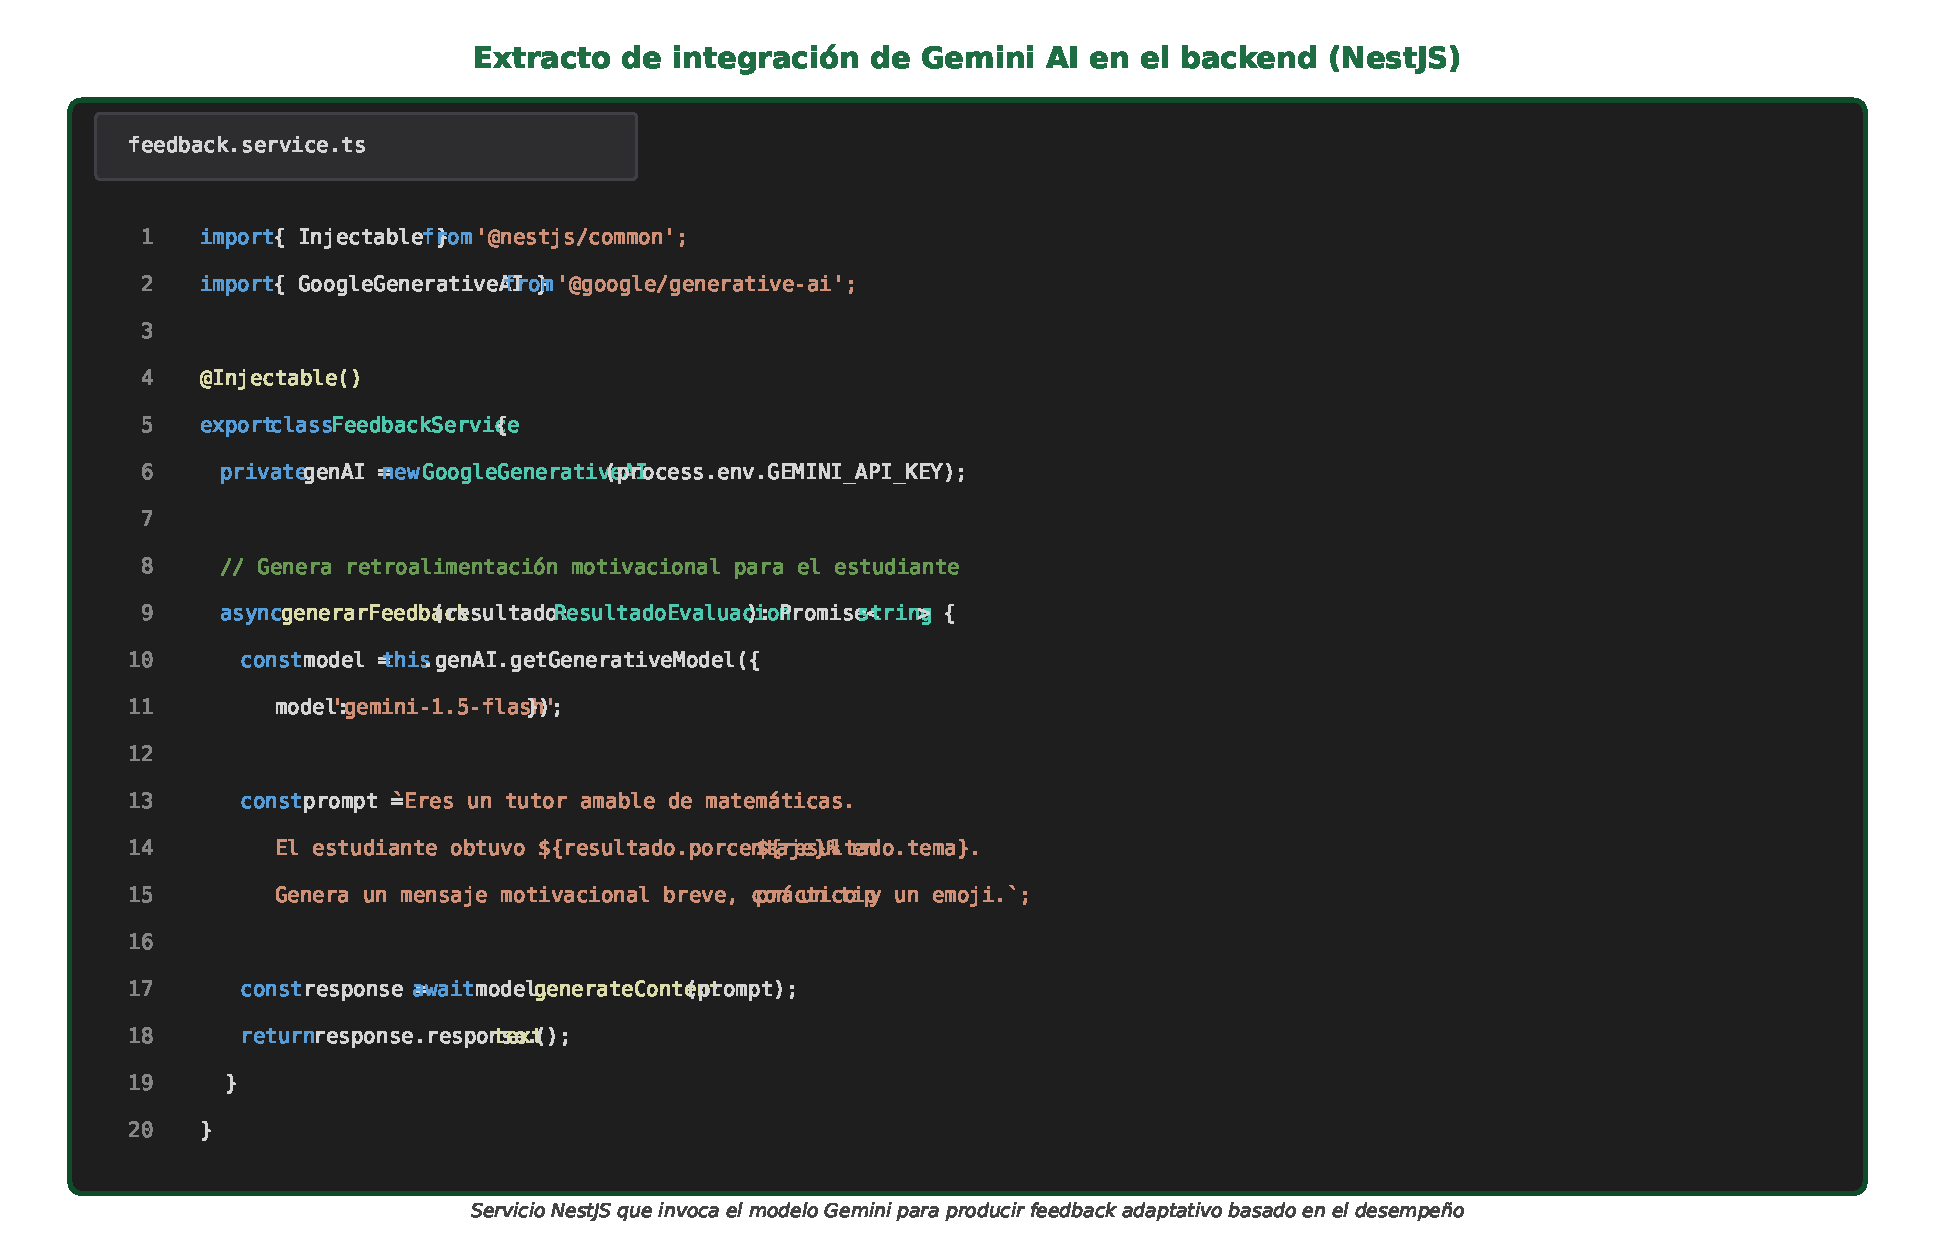
\includegraphics[width=\textwidth]{figuras/fig09_gemini_ai.pdf}
\fuenteautor
\end{figure}

Para este propósito se configuró el entorno utilizando el modelo \textbf{Gemini 1.5 Flash} de Google. A diferencia de las plataformas que ofrecen calificaciones estáticas, esta arquitectura permite procesar el desempeño del estudiante en tiempo real. Como se observa en el bloque de código, el sistema filtra los datos de la evaluación y construye un \textit{prompt} estructurado donde la inteligencia artificial asume el rol de un asistente académico. Las instrucciones programadas exigen que el modelo devuelva un reporte exhaustivo en formato Markdown, el cual incluye obligatoriamente: información general de la participación, resultados detallados por pregunta, análisis de fortalezas, identificación de áreas de oportunidad y recomendaciones académicas. Esta configuración asegura que el estudiante no solo reciba una nota, sino una retroalimentación formativa, automatizada y contextualizada, fundamental para el fortalecimiento de las competencias matemáticas.

\subsection{Seguridad y autenticación}

Para garantizar la integridad de la información y la privacidad de los usuarios, la plataforma implementa un modelo de seguridad basado en JSON Web Tokens (JWT), gestionado centralmente desde el \textit{backend} con el \textit{framework} NestJS. En la Ilustración~\ref{fig:jwt} se detalla el flujo de autenticación adoptado por el sistema. El proceso inicia cuando el usuario ingresa sus credenciales, las cuales son validadas comprobando el \textit{hash} de la contraseña contra la base de datos PostgreSQL. Tras una validación exitosa, el servidor emite un token JWT firmado criptográficamente, el cual es almacenado en el cliente y utilizado en el encabezado de autorización (esquema \textit{Bearer}) en las peticiones subsecuentes.

\begin{figure}[H]
\centering
\caption{Flujo de autenticación por JWT en Kiddy Quiz.}
\label{fig:jwt}
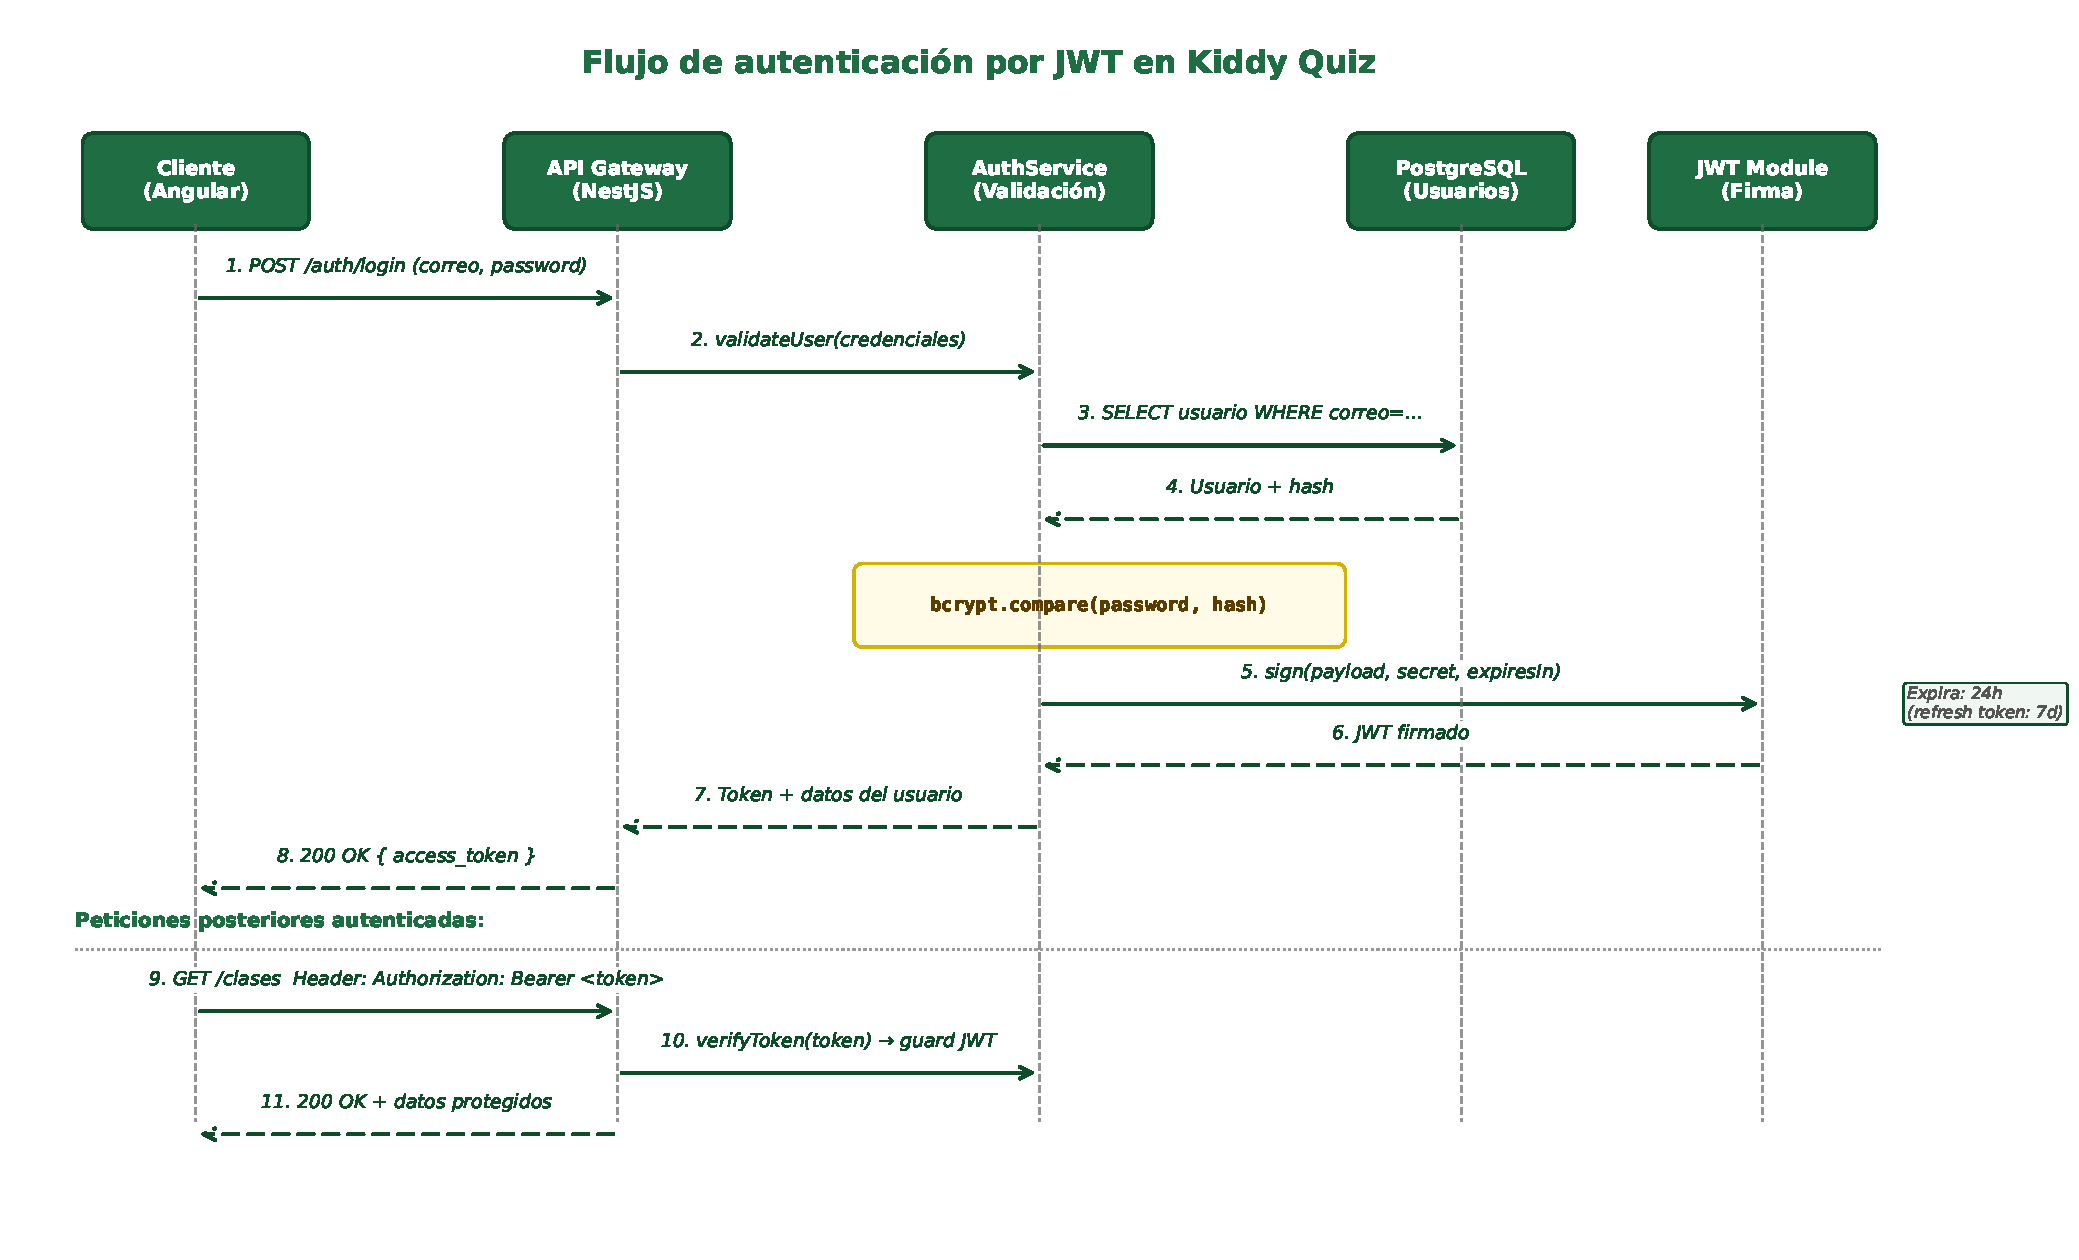
\includegraphics[width=\textwidth]{figuras/fig10_jwt.pdf}
\fuenteautor
\end{figure}

Este mecanismo de tokens no solo protege las sesiones, sino que fundamenta el control de acceso basado en roles (RBAC) del sistema. Al interceptar la petición y extraer el \textit{payload} con métodos de verificación, el \textit{backend} identifica de manera inmediata si la petición proviene de un perfil de estudiante o de un docente, restringiendo los permisos en las rutas de la API. En caso de detectar un token inválido o permisos insuficientes, el sistema deniega el acceso retornando los códigos de estado HTTP correspondientes (401 No autorizado o 403 Acceso prohibido).

\section{Comprobación}

En esta sección se presenta la validación integral del proyecto tecnológico desarrollado, evidenciando su correcto funcionamiento y evaluando su desempeño en función de los indicadores de evaluación previamente establecidos en la sección~3.5. Estos parámetros fueron definidos para asegurar que Kiddy Quiz cumpla con los requerimientos pedagógicos y técnicos iniciales, permitiendo medir de forma objetiva su calidad, su rendimiento técnico y su nivel de aceptación por parte de los usuarios.

\subsection{Cumplimiento de plazos}

En la Ilustración~\ref{fig:plazos} se expone una comparativa detallada entre las fechas establecidas inicialmente en la planificación del proyecto y las fechas efectivas en las que se dio cumplimiento a cada uno de los hitos. Cabe destacar que, debido a la naturaleza iterativa de la metodología ágil de Programación Extrema, el cronograma mantuvo un enfoque flexible. En consecuencia, las fechas de finalización de ciertos módulos experimentaron ligeros ajustes con el propósito de incorporar correcciones, mejoras de usabilidad y refactorizaciones de código, garantizando así la calidad del producto final dentro de las treinta y dos semanas estipuladas.

\begin{figure}[H]
\centering
\caption{Cumplimiento de plazos por fase del proyecto Kiddy Quiz.}
\label{fig:plazos}
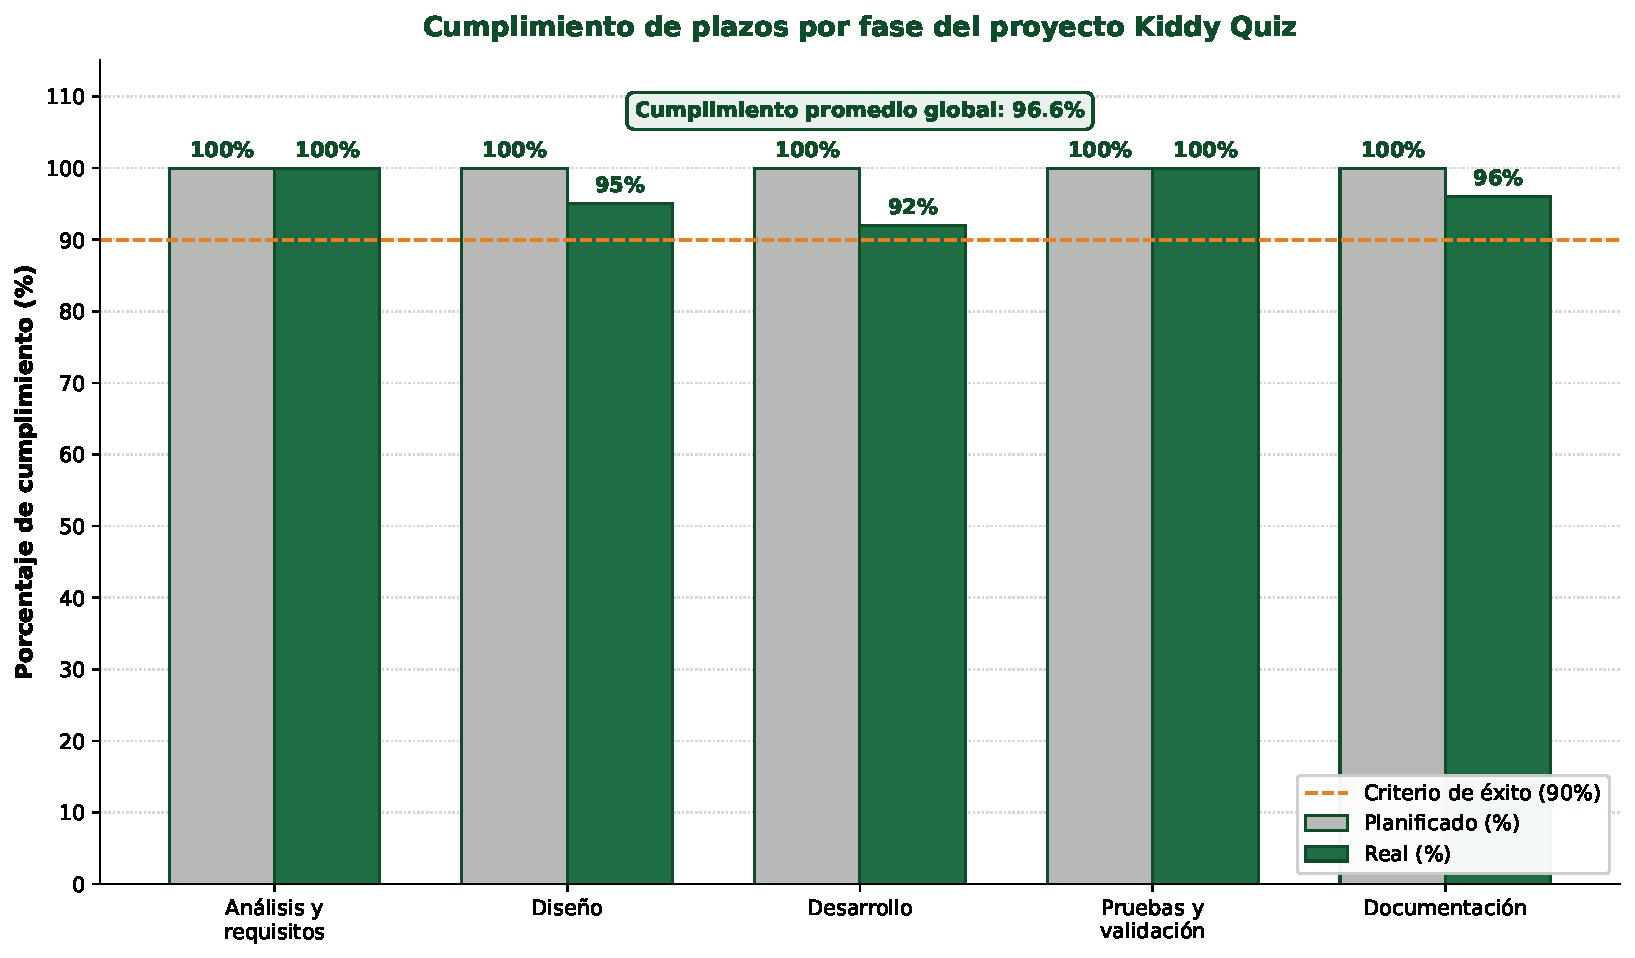
\includegraphics[width=0.95\textwidth]{figuras/fig11_cumplimiento_plazos.pdf}
\fuenteautor
\end{figure}

El cumplimiento promedio global se situó en 96,6\,\%, superando holgadamente el criterio mínimo de 90\,\% establecido en la Tabla~\ref{tab:ind_plazos}.

\subsection{Nivel de aceptación de usuario}

El análisis del nivel de usabilidad y aceptación tecnológica de la plataforma Kiddy Quiz se llevó a cabo mediante la aplicación de la Escala de Usabilidad del Sistema (SUS) y el Modelo de Aceptación Tecnológica (TAM). Estos instrumentos permitieron evaluar de forma objetiva la facilidad de interacción, la utilidad pedagógica percibida y la experiencia general tanto de los estudiantes como de los docentes al utilizar la aplicación. Los resultados consolidados de ambas pruebas demuestran que el sistema no solo cumple satisfactoriamente con las expectativas de los usuarios, sino que facilita un entorno educativo altamente funcional e intuitivo.

\subsubsection{Resultados de las evaluaciones de usabilidad (SUS)}

Para evaluar de manera exhaustiva la usabilidad de la plataforma se aplicó la Escala de Usabilidad del Sistema (SUS). El análisis descriptivo de los datos recopilados, segmentado por los dos grupos principales de usuarios (docentes y estudiantes), demuestra un nivel de accesibilidad y diseño excepcional. Como se detalla en la Tabla~\ref{tab:sus}, las métricas de tendencia central reflejan un desempeño sobresaliente. El grupo de estudiantes otorgó una calificación promedio de 87,7 sobre 100, con una mediana de 87,5, lo que evidencia una interacción sumamente fluida e intuitiva. Por su parte, el grupo de docentes registró una media favorable de 81,0 y una mediana de 82,5.

\begin{table}[H]
\centering
\caption{Resultados del cuestionario SUS aplicado a Kiddy Quiz.}
\label{tab:sus}
\begin{tabularx}{\textwidth}{|L{4.5cm}|C{3cm}|C{3cm}|}
\hline
\rowcolor{tabhead}
\tabhead{Métrica estadística} & \tabhead{Estudiantes (N=15)} & \tabhead{Docentes (N=5)}\\
\hline
Media & 87,7 & 81,0\\
\hline
Mediana & 87,5 & 82,5\\
\hline
Desviación estándar & 7,8 & 9,4\\
\hline
Valor mínimo & 80,0 & 67,5\\
\hline
Valor máximo & 95,0 & 95,0\\
\hline
\end{tabularx}
\fuenteautor
\end{table}

Resulta fundamental destacar el valor mínimo obtenido en la muestra de estudiantes, el cual se situó en 80,0. Este dato estadístico es de vital importancia, ya que confirma que ningún niño experimentó dificultades severas al navegar por los módulos o al momento de resolver sus evaluaciones. Asimismo, las desviaciones estándar (7,8 para estudiantes y 9,4 para docentes) sugieren un consenso generalizado sobre la calidad de la experiencia de usuario, superando holgadamente el puntaje de 68,0 considerado como el estándar mínimo aceptable en la industria.

Con el propósito de ilustrar el posicionamiento de estos resultados frente a los estándares internacionales de usabilidad, la Ilustración~\ref{fig:sus} despliega un gráfico de barras que contrasta las puntuaciones medias obtenidas. En esta representación visual se aprecia claramente cómo ambos perfiles de usuario superan la línea base de los 68 puntos, ubicándose firmemente dentro de la zona de aceptabilidad y excelencia.

\begin{figure}[H]
\centering
\caption{Resultados del cuestionario SUS – Aplicación Kiddy Quiz.}
\label{fig:sus}
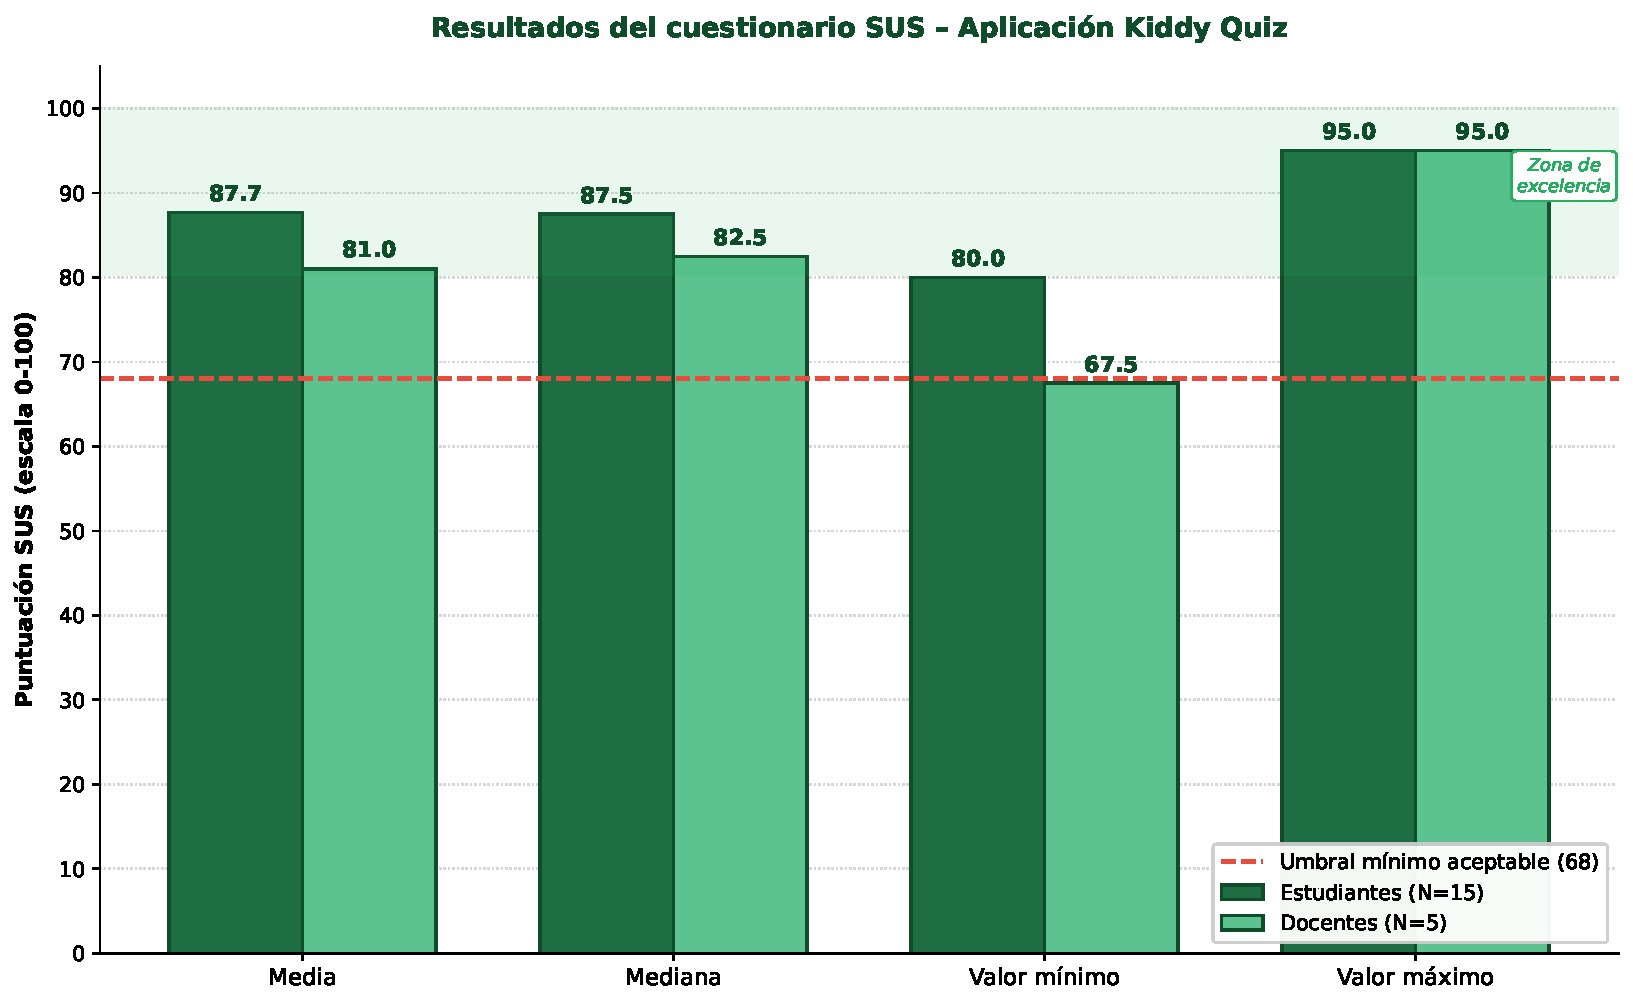
\includegraphics[width=0.95\textwidth]{figuras/fig12_grafico_sus.pdf}
\fuenteautor
\end{figure}

\subsubsection{Resultados del Modelo de Aceptación Tecnológica (TAM)}

Para complementar la evaluación de usabilidad se aplicó el Modelo de Aceptación Tecnológica (TAM), con el objetivo de medir empíricamente la viabilidad pedagógica y el nivel de adopción de la plataforma. Este instrumento evalúa tres dimensiones fundamentales: la Utilidad Percibida (PU), la Facilidad de Uso Percibida (PEOU) y la Intención de Uso (IU), valoradas mediante una escala de Likert de 1 a 5.

El análisis descriptivo de las respuestas, estructurado por tipo de usuario, revela una aceptación excepcional de la herramienta, destacando una tendencia sumamente positiva por parte del grupo de estudiantes. Al observar los estadísticos de tendencia central se evidencia que los niños perciben una mayor facilidad al navegar por la plataforma (media de 4,78) en comparación con los docentes (media de 3,95). Este contraste valida contundentemente la eficacia del diseño de interfaz centrado en el usuario infantil: el uso de pictogramas y elementos visuales simplificados logró que los estudiantes interactuaran con el sistema de forma más natural e intuitiva que los propios adultos. Asimismo, la baja desviación estándar en las métricas de los estudiantes (oscilando entre 0,14 y 0,23) indica un alto grado de consenso, confirmando que la experiencia positiva fue generalizada y no un caso aislado.

El hallazgo más significativo dentro de esta evaluación recae en la dimensión de Intención de Uso. El grupo de estudiantes registró una media de 4,93 y una mediana perfecta de 5,0, con un valor mínimo de 4,6. Esta calificación, que roza el límite superior absoluto de la escala, demuestra un nivel de motivación intrínseca sobresaliente, atribuible directamente a la innovación central del proyecto: la integración de retroalimentación generada por Inteligencia Artificial.

\begin{table}[H]
\centering
\caption{Resultados del cuestionario TAM aplicado a Kiddy Quiz.}
\label{tab:tam}
\begin{small}
\begin{tabularx}{\textwidth}{|L{3.7cm}|L{2.7cm}|C{1.4cm}|C{1.6cm}|X|}
\hline
\rowcolor{tabhead}
\tabhead{Dimensión} & \tabhead{Grupo} & \tabhead{Media} & \tabhead{Desv.~Est.} & \tabhead{Interpretación}\\
\hline
\multirow{2}{*}{Utilidad Percibida (PU)} & Docentes (N=5) & 4,45 & 0,33 & Muy alta percepción de utilidad pedagógica\\
\cline{2-5}
 & Estudiantes (N=15) & 4,85 & 0,22 & Percepción cercana al máximo absoluto\\
\hline
\multirow{2}{*}{Facilidad de Uso (PEOU)} & Docentes (N=5) & 3,95 & 0,27 & Facilidad alta, requiere mínimo esfuerzo\\
\cline{2-5}
 & Estudiantes (N=15) & 4,78 & 0,23 & Interfaz extremadamente intuitiva\\
\hline
\multirow{2}{*}{Intención de Uso (IU)} & Docentes (N=5) & 4,47 & 0,38 & Fuerte disposición a integrar la herramienta\\
\cline{2-5}
 & Estudiantes (N=15) & 4,93 & 0,14 & Intención casi unánime y máxima\\
\hline
\end{tabularx}
\end{small}
\fuenteautor
\end{table}

Para ilustrar de manera visual y comparativa los resultados estadísticos expuestos, la Ilustración~\ref{fig:tam} presenta un gráfico de brechas (\textit{Dumbbell Plot}) enfocado en las tres dimensiones del Modelo TAM. Esta representación gráfica permite contrastar de forma directa las puntuaciones medias otorgadas por docentes y estudiantes.

\begin{figure}[H]
\centering
\caption{Gráfico de brechas TAM – Comparación docentes vs.\ estudiantes.}
\label{fig:tam}
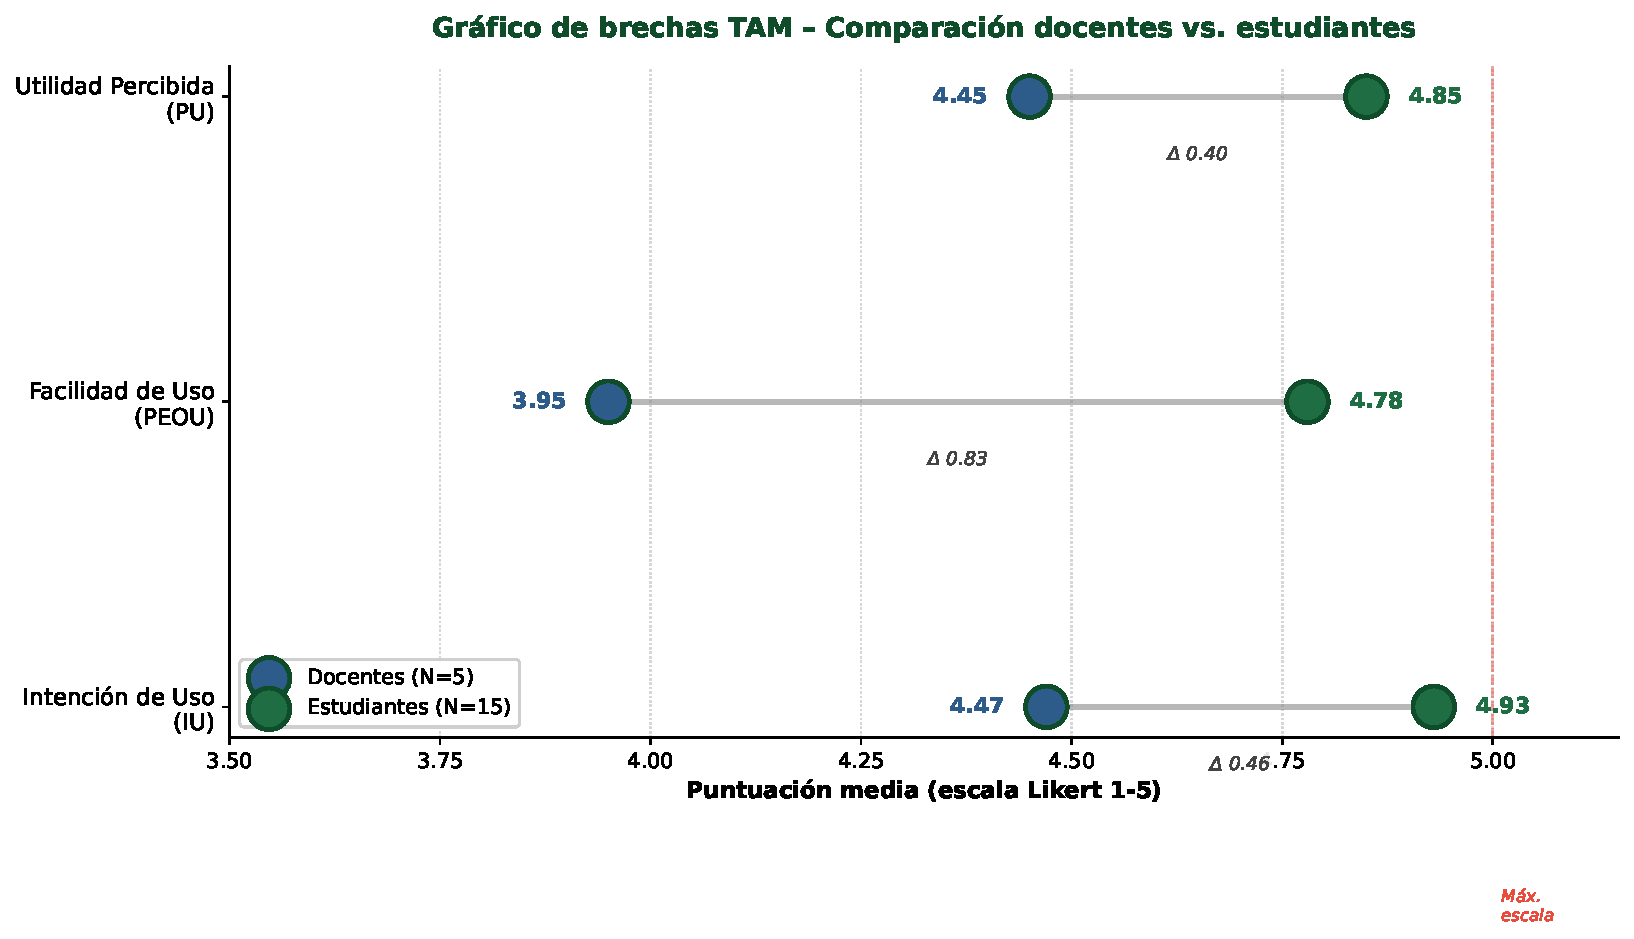
\includegraphics[width=0.95\textwidth]{figuras/fig13_grafico_tam.pdf}
\fuenteautor
\end{figure}

Como se puede observar en el gráfico, la longitud de las líneas conectoras evidencia la diferencia de percepción entre ambos perfiles de usuario. La brecha más amplia se presenta claramente en la Facilidad de Uso (PEOU), donde los estudiantes (4,78) superan de forma notoria a los docentes (3,95). Esto demuestra gráficamente que la interfaz adaptada cumplió su objetivo de reducir la carga cognitiva en los niños. Asimismo, la gráfica destaca cómo el indicador de Intención de Uso en los estudiantes alcanza el punto máximo del esquema (4,93), posicionándose casi en el límite perfecto de la escala. En conjunto, esta visualización corrobora que Kiddy Quiz logró una adopción tecnológica sobresaliente, validando el impacto positivo de la inteligencia artificial y el diseño interactivo en el público infantil.

\section{Discusión}

Los resultados obtenidos confirman la pertinencia y eficacia de la solución propuesta, en línea con la literatura existente sobre evaluación por competencias y tecnologías educativas. La puntuación SUS de 87,7 obtenida con los estudiantes ubica a Kiddy Quiz en la categoría de \textit{Excelente} según la escala de Bangor, superando los rangos típicamente reportados para herramientas similares orientadas a educación superior \cite{ref10_cat,ref21_scala_universidad}. Resulta particularmente significativa la diferencia entre la facilidad de uso percibida por los estudiantes (4,78) y la de los docentes (3,95): mientras la literatura suele reportar mayor dificultad de uso en niños debido a su menor experiencia tecnológica, en este caso el resultado se invierte gracias al diseño centrado en pictogramas y elementos visuales simplificados \cite{ref40_mayer,ref48_nielsen}, una validación empírica del principio de doble codificación \cite{ref43_paivio}.

Comparado con SCALA \cite{ref21_scala_universidad}, CAT \cite{ref10_cat} y SECAT \cite{ref11_secat}, Kiddy Quiz introduce tres diferenciadores sustantivos que constituyen su aporte original: (i) el enfoque deliberado en educación básica elemental --un nivel desatendido en la literatura existente--; (ii) la integración de retroalimentación generativa por IA, que trasciende las rúbricas estáticas de los antecedentes; y (iii) la incorporación nativa de elementos de accesibilidad visual, alineada con las recomendaciones de equidad educativa \cite{ref42_cabero}. Estos hallazgos refuerzan la tesis de que la digitalización efectiva en evaluación educativa requiere no solo plataformas funcionales, sino diseños pedagógicamente situados y empíricamente validados \cite{ref14_anderson,ref27_blackwiliam}.

Las brechas observadas entre la percepción de docentes y estudiantes coinciden con los hallazgos de Ertmer y Ottenbreit-Leftwich \cite{ref08_ertmer} sobre las barreras de adopción tecnológica del profesorado, lo que sugiere la necesidad de complementar el producto con instancias de capacitación docente. No obstante, la alta intención de uso reportada por los docentes (4,47) indica una disposición favorable hacia la incorporación de la herramienta en sus prácticas, especialmente cuando los beneficios de automatización del seguimiento académico se hacen tangibles.
